\chapter{Quality of experience evaluation}
\label{cha:eval}

In this section, we will use the testbed presented in the previous chapter to execute some \textbf{experiments} and highlight some of the issues of current streaming technologies in low-latency scenarios. We will present how the data collected through the testbed is visualized and show some of the most important results and observations.

The results of the evaluation will be the basis for the improvements proposed in Chapter \ref{cha:improvements}.

\section{Different browsers behaviors}
\label{sec:eval/browsers}

An important thing to keep in mind when evaluating the performance of streaming protocols is that different browsers have different implementations of the network protocols and can therefore show different behaviors. One of these differences relates to how \textbf{HTTP priorities} are handled.

\subsection{HTTP priorities handling in Chromium and Firefox}
\label{sec:eval/browsers/priorities}

According to our tests, Chromium (v107) allows to specify the \texttt{Priority} header in requests sent with the \texttt{fetch} API or with \texttt{XMLHttpRequest}. The header is in fact passed as is to the HTTP server and is correctly interpreted by servers supporting the extensible priorities specification (Section \ref{sec:bg/http3}). However, the browser also sends a \texttt{PRIORITY\_UPDATE} frame after sending the HTTP request, overriding the priority specified through the header. The \texttt{PRIORITY\_UPDATE} frame is sent as part of the prioritization strategy implemented by the browser, which applies its own heuristics to determine which requests should be prioritized, both internally in the browser and at the network level.

The \textbf{Priority Hints} feature provides a way to control the priority that the browser gives to individual HTTP requests. The Priority Hints specification is still a W3C draft, but Chromium already implements it. The priority values defined by the specification are \texttt{high} and \texttt{low}.\footnote{\url{https://wicg.github.io/priority-hints/}} By default, \texttt{fetch} API requests have a priority of \texttt{high}, which corresponds to HTTP/3 priority \texttt{1} (where \texttt{0} means highest priority), transmitted in the \texttt{PRIORITY\_UPDATE} frame. If the \texttt{fetch} priority is set to \texttt{low}, it turns out that Chromium does not send the \texttt{PRIORITY\_UPDATE} frame at all, effectively leaving the priority value at the default value of \texttt{3}. As a consequence, in practice, setting the fetch priority to \texttt{low} enables setting a custom priority through the \texttt{Priority} header. Figure \ref{fig:chromium_fetch} shows some examples of how priorities are currently handled in Chromium.

\begin{figure}[h]
    \centering
    \begin{minted}[frame=single]{js}
await fetch('/');
// Priority hint   => default => high
// Priority header => not sent
// PRIORITY_UPDATE => sent with urgency 1

await fetch('/', { headers: { Priority: 'u=2' } });
// Priority hint   => default => high
// Priority header => sent with urgency 2
// PRIORITY_UPDATE => sent with urgency 1

await fetch('/', { priority: 'low' });
// Priority hint   => low
// Priority header => not sent
// PRIORITY_UPDATE => not sent, default to urgency 3

await fetch('/', { priority: 'low', headers: { Priority: 'u=2' } });
// Priority hint   => low
// Priority header => sent with urgency 2
// PRIORITY_UPDATE => not sent
    \end{minted}
    \caption{Summary of the observed behaviors when trying to set custom HTTP/3 priorities in Chromium.}
    \label{fig:chromium_fetch}
\end{figure}

In summary, \textbf{in Chromium it is possible to set custom priority values} by using the \texttt{Priority} header, the Priority Hints feature, or a combination of the two.

In Firefox (v107), the behavior is different. First, Firefox does not support Priority Hints. It also appears that it does not use the \texttt{PRIORITY\_UPDATE} frame, instead adding the \texttt{Priority} header internally to outgoing requests. By default, the urgency is set to \texttt{4} for \texttt{fetch} requests. However, manually setting the \texttt{Priority} header does not seem to have any effect, as the header is always overridden by Firefox. In practice, this means that \textbf{until Firefox adds support for Priority Hints there does not seem to be a way to send a custom priority}.

\subsection{The issue with CORS}
\label{sec:eval/browsers/cors}

A problem that might arise when using the \texttt{Priority} header, common to all browsers, is related to how \textbf{cross-origin requests} are handled.

A cross-origin request is a request generated by a web page that has a destination whose domain, scheme, or port do not match those of the current web page. For security reasons, browsers require that the server explicitly authorizes the origin to execute cross-origin requests when they might have undesired effects on user data. This is done through CORS, which consists in sending an additional preflight request before the actual HTTP request so that the server can specify which requests are allowed (through response headers).

The presence of the \texttt{Priority} header triggers a preflight request before each HTTP request if the request is cross-origin (which is often the case when using a CDN). Unfortunately, this additional request can introduce significant latency.

\subsection{The h2o patch}
\label{sec:eval/browsers/patch}

To work around the issue of not being able to specify the HTTP/3 priority in some cases, and more importantly the CORS issue, we implemented a patch to \texttt{h2o} so that the priority can be forced with a query string parameter.\footnote{\url{https://github.com/matteocontrini/h2o/commit/bf307ef}} So, for example, a request like \texttt{GET /segment.m4s?priority=2} would give the request an urgency value of \texttt{2}.

\section{Experiments and results with non-ABR setup}
\label{sec:eval/non-abr}

As a first experiment with our testbed, we investigated how video streaming behaves when the network bandwidth is unstable and the bitrate is fixed, i.e. no bitrate adaptation is carried out. As we shall see, although this situation is not realistic, it allows us to better observe the different behaviors between HTTP versions.

We based this first analysis on \textbf{MPEG-DASH} with the \dashjs{} library, with a \textbf{target live latency of 4 seconds}, corresponding to 2 segments. The bitrate of the video rendition is the highest one, i.e. 3.5 Mbps.

For this setup, we used network patterns from the 4G dataset. Specifically, the \texttt{lte} and \texttt{hspa+} patterns, as seen in Section \ref{sec:testbed/network/patterns}. The average RTT is set to 80 ms with a jitter of 15 ms.

For each of these two patterns, we tested how the system behaves with HTTP/1.1, HTTP/2 and HTTP/3. For HTTP/3, we also tested with the live catchup feature enabled. In practice, this means that 8 experiments were defined, as shown in Figure \ref{fig:experiments1}.

\begin{figure}[h]
    \centering
    \begin{minted}[frame=single,fontsize=\small]{js}
const experiments = [
  new Experiment('lte_h1', 'lte', ABRProtocol.DASH, HttpVersion.HTTP1_1, 3000),
  new Experiment('lte_h2', 'lte', ABRProtocol.DASH, HttpVersion.HTTP2, 3000),
  new Experiment('lte_h3', 'lte', ABRProtocol.DASH, HttpVersion.HTTP3, 3000),
  new Experiment('hspa+_h1', 'hspa+', ABRProtocol.DASH, HttpVersion.HTTP1_1, 3000),
  new Experiment('hspa+_h2', 'hspa+', ABRProtocol.DASH, HttpVersion.HTTP2, 3000),
  new Experiment('hspa+_h3', 'hspa+', ABRProtocol.DASH, HttpVersion.HTTP3, 3000),
  new Experiment('lte_catchup', 'lte', ABRProtocol.DASH, HttpVersion.HTTP3, 3000, true),
  new Experiment('hspa+_catchup', 'hspa+', ABRProtocol.DASH, HttpVersion.HTTP3, 3000, true)
];
    \end{minted}
    \caption{TypeScript code showing how the list of experiments is defined in the testbed.}
    \label{fig:experiments1}
\end{figure}

\subsection{Suboptimal behavior over HTTP/3}
\label{sec:eval/non-abr/h3-behavior}

As a first step, we will look at the results of the experiment named \texttt{lte\_h3}, which uses DASH over HTTP/3 with the \texttt{lte} dataset.

The \textbf{buffer health plot} is shown in Figure \ref{fig:eval_nonabr_lte_h3}. In detail, the elements of the plot have the following meaning:

\begin{itemize}
    \item The gray area in the background represents the \textbf{network bandwidth}, with the Mbps scale shown on the right side. As we can see, it varies between about 2 and 16 Mbps over the duration of the experiments, which is approximately 60 seconds with this network pattern.
    \item The orange line represents the \textbf{bitrate of the media}, calculated as the sum of the video and audio bitrates. In this case, it is constant at about 3.5 Mbps.
    \item The black line indicates the \textbf{size of the video buffer in seconds}. The scale is shown to the left of the panel.
    \item The purple line instead refers to the \textbf{audio buffer size}.
    \item The vertical dotted lines refer to the \textbf{buffer events}. The red lines correspond to empty buffer events (for any track), while the green lines indicate buffer loaded.
    \item The red areas between the dotted lines represent the \textbf{playback stalls}. The left border of a red area corresponds to a playback stalled event, while the right border corresponds to playback resumption.
\end{itemize}

\begin{figure}[h]
    \centering
    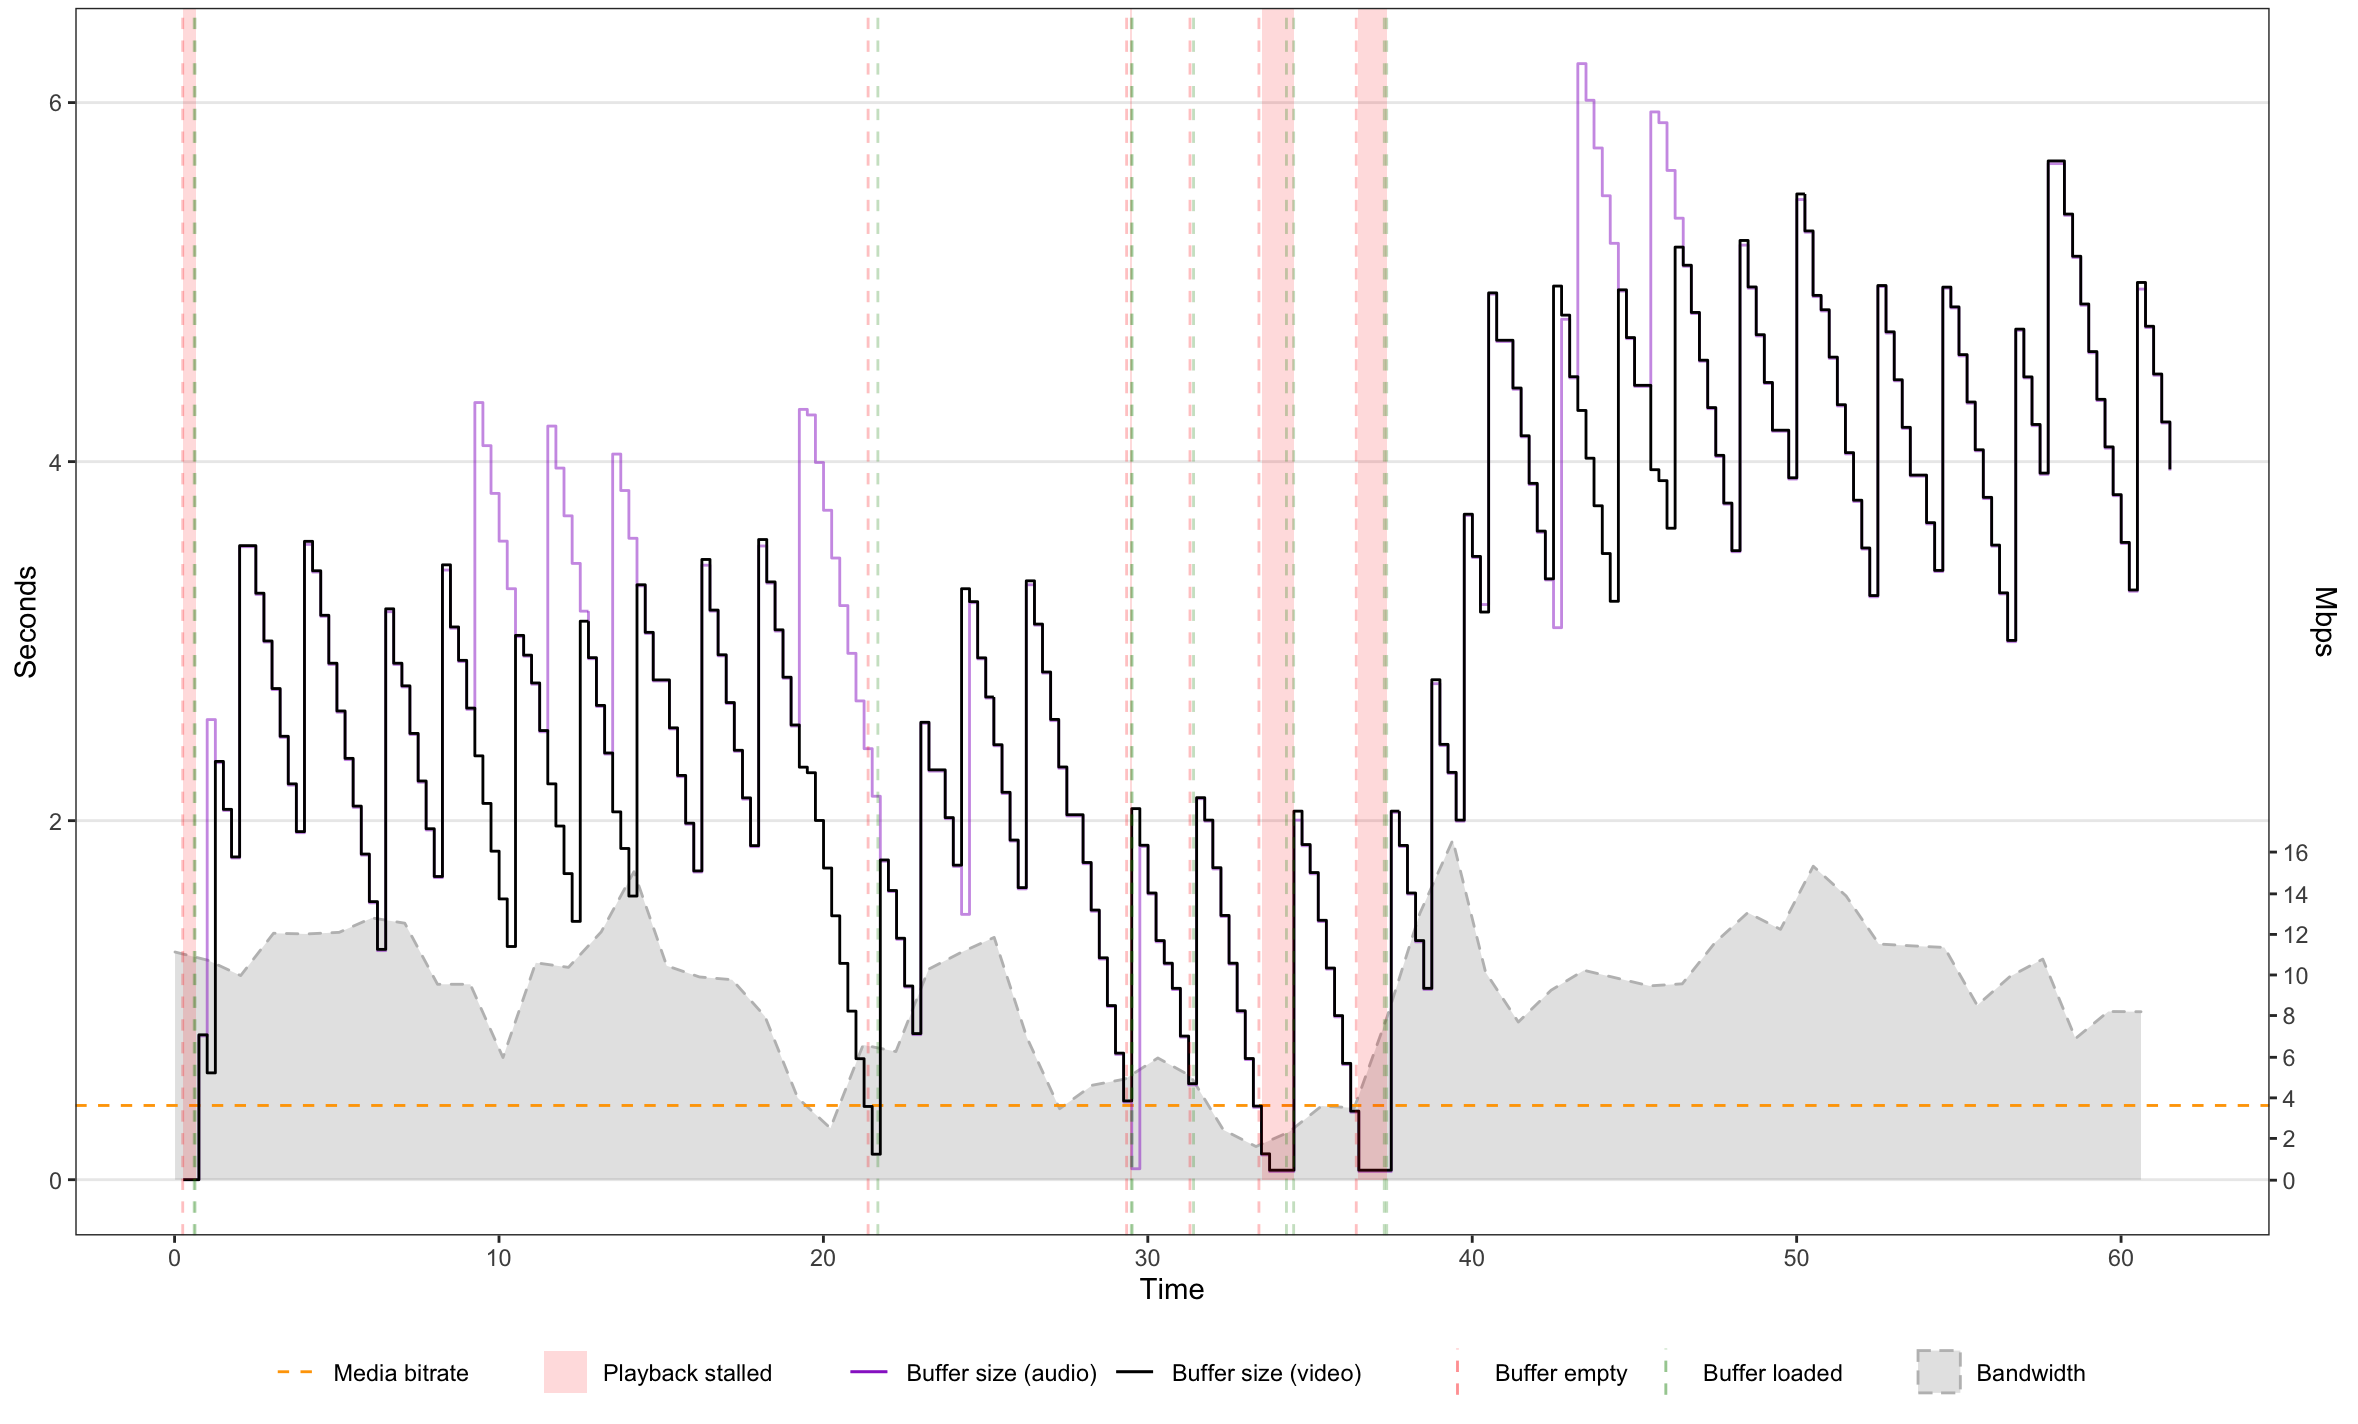
\includegraphics[width=\textwidth]{res/eval_nonabr_lte_h3.png}
    \caption{Buffer health plot for DASH with the \texttt{lte} network pattern over HTTP/3.}
    \label{fig:eval_nonabr_lte_h3}
\end{figure}

What we can observe from the plot is that for the first 30 seconds the bandwidth is generally above the bitrate of the media, and therefore the buffer can be filled properly most of the time. Another observation that we can already make is that the audio buffer is sometimes filled with more seconds of data than the video buffer. This happens because \textbf{the video and audio tracks are unmuxed and can therefore be downloaded independently} by the player/browser. Depending on the HTTP response scheduling, the audio segment might arrive before the video segment, or vice versa.

In the first half of the experiment, we can also notice a couple of cases where the player struggles to fill the video buffer in time. For example, just after second 20 the video buffer actually becomes empty for a very short period of time. As we will see later, in practice this kind of event does not necessarily produce a playback stall due to the way Chromium handles empty buffers.

At about second 30, the bandwidth starts to become very limited and goes below 3.5 Mbps for a few seconds. The video and audio buffers quickly deplete, empty buffer events are emitted, and the playback stalls. This happens twice, as can be seen by the two red areas.

When the network bandwidth grows again, the buffers are filled. One thing to note is that the buffer length now contains about one segment more on average (it is in fact closer to 4 seconds than to 2). This happens because the delay introduced by the stall caused the playback to get behind with respect to the edge of the playlist, and therefore there is now an additional segment that can be loaded in advance.

The effect of this behavior can be better seen in the \textbf{live latency plot}, shown in Figure \ref{fig:eval_nonabr_lte_h3_latency}. In correspondence of the playback stalls, the live latency grows from about 4.5 to 5.5 seconds, and then to 6.5 seconds (in total, a 2-second segment more).

\begin{figure}[h]
    \centering
    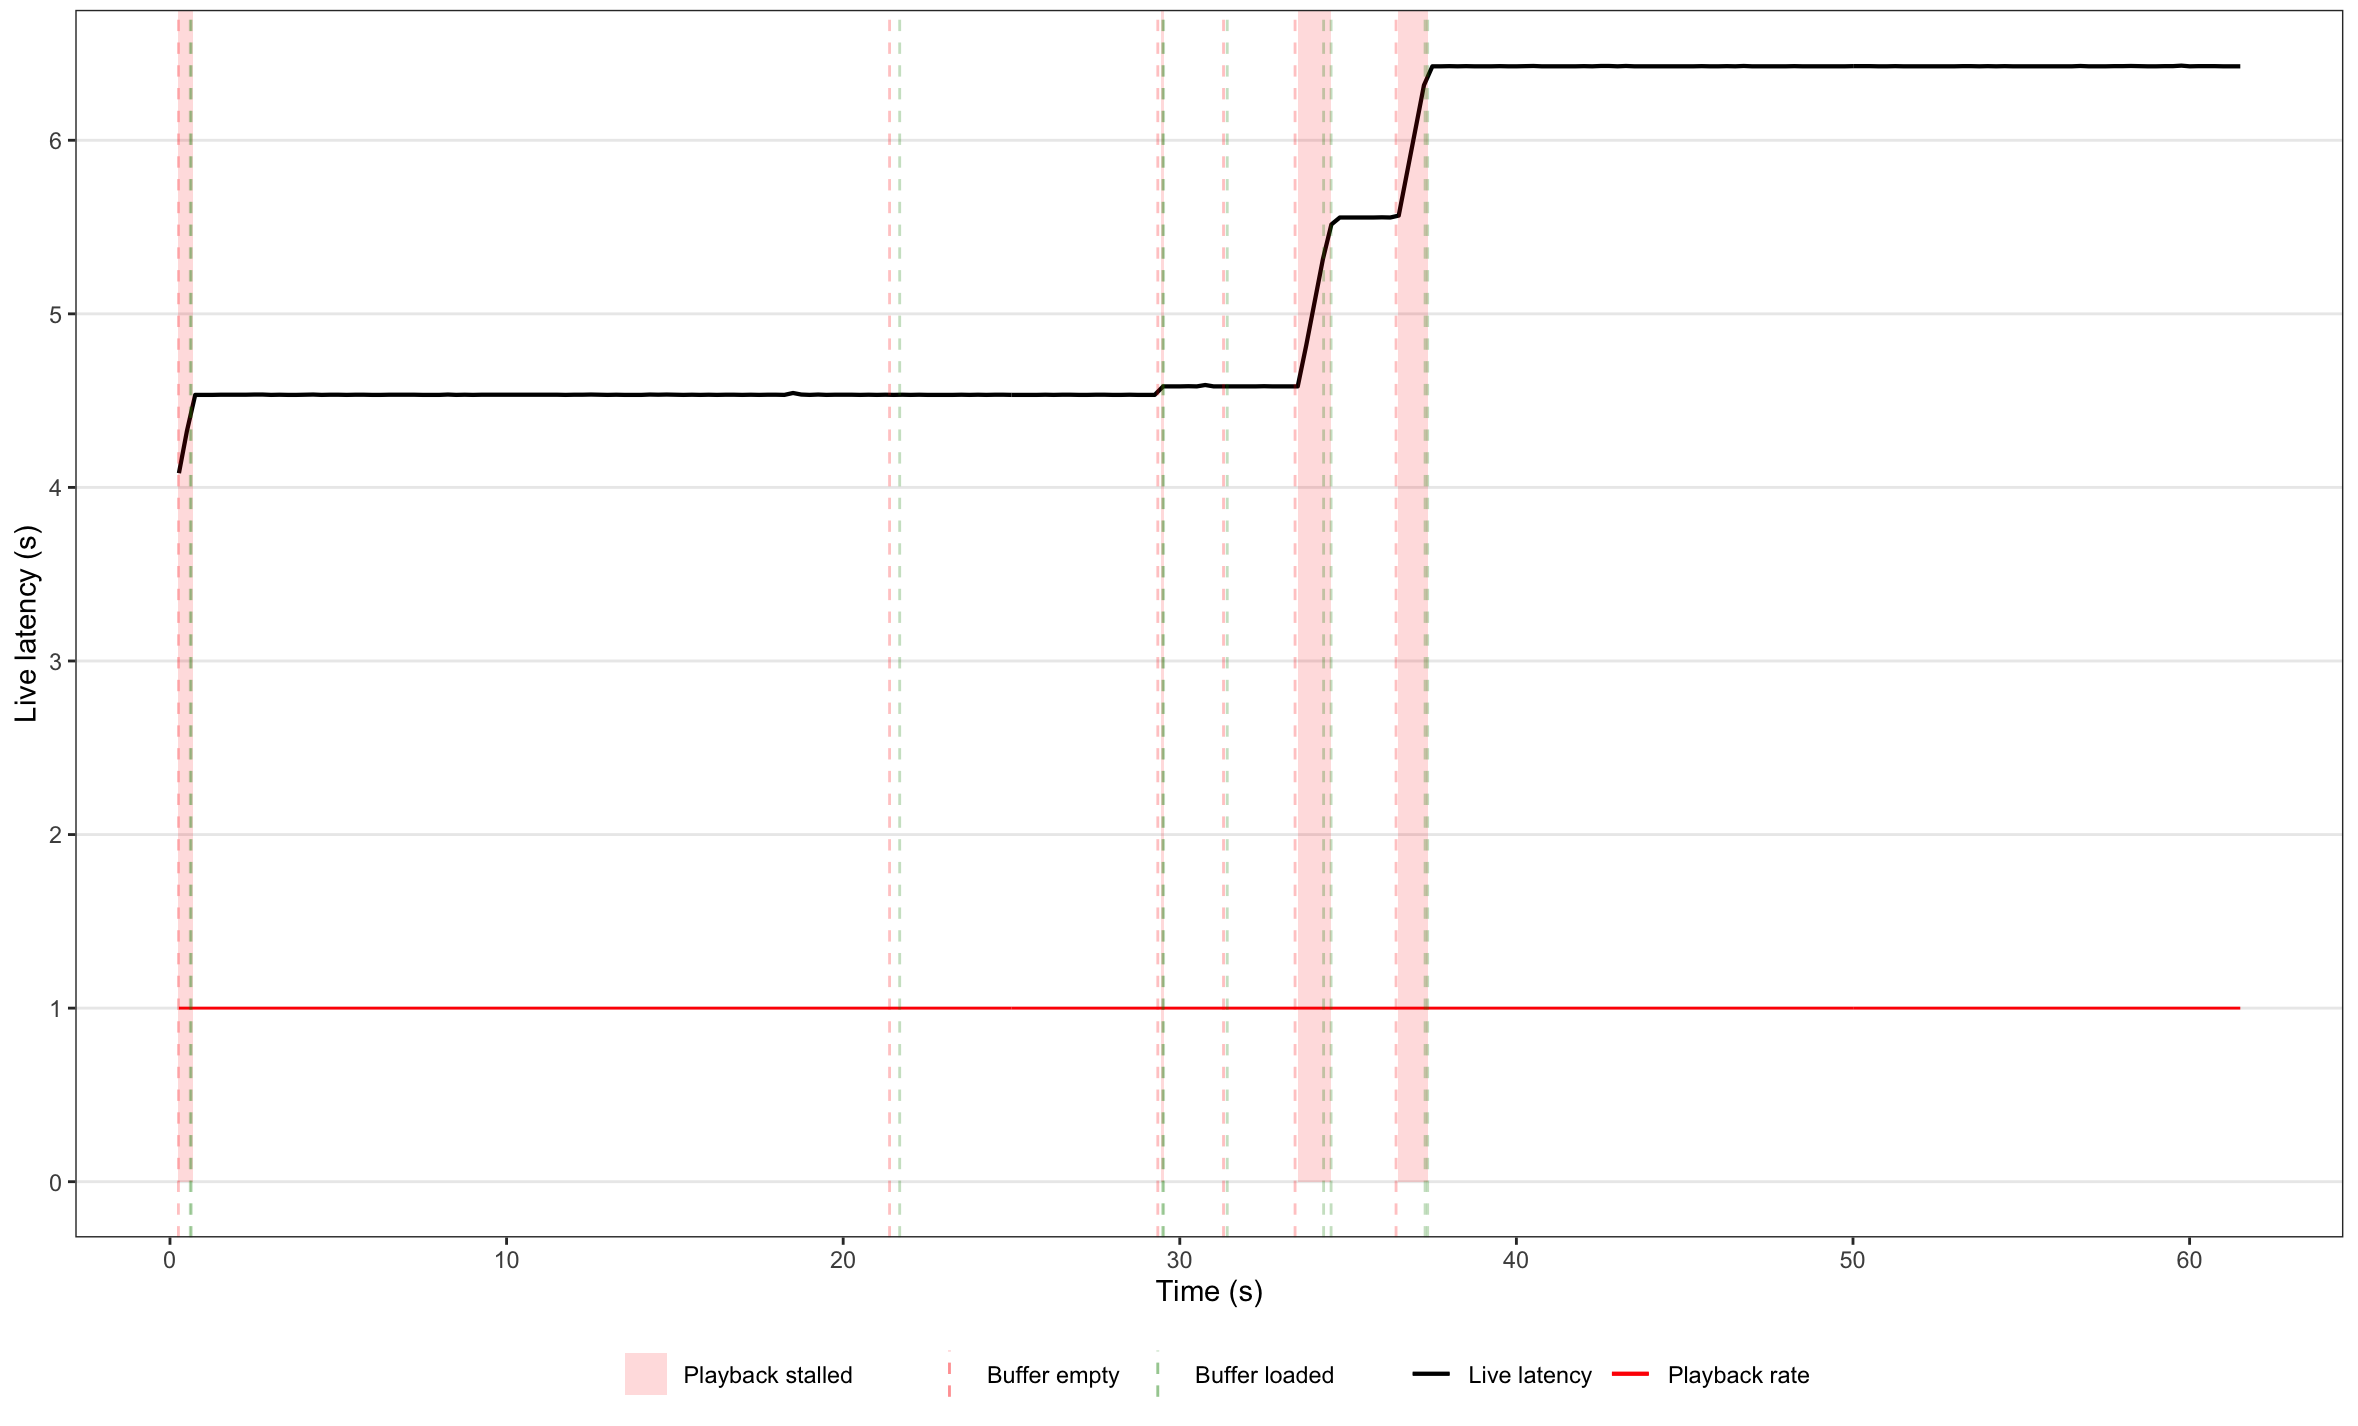
\includegraphics[width=0.9\textwidth]{res/eval_nonabr_lte_h3_latency.png}
    \caption{Live latency plot for DASH with the \texttt{lte} network pattern over HTTP/3.}
    \label{fig:eval_nonabr_lte_h3_latency}
\end{figure}

Finally, if we observe the \textbf{waterfall diagram} (Figure \ref{fig:eval_nonabr_lte_h3_waterfall}), an interesting and perhaps unexpected behavior can be observed. Intuitively, we would expect requests for audio segments to always take less time than video segments. In fact, while a single video segment can be as large as 6-700 KiB, the audio segment is usually about 30 KiB in size. This means that \textbf{audio is approximately between 10 and 20 times smaller than video}. However, the waterfall shows that, while sometimes the loading of the audio segment takes very little time, \textbf{the loading of the audio segments often takes as long as the video}.

\begin{figure}[h]
    \centering
    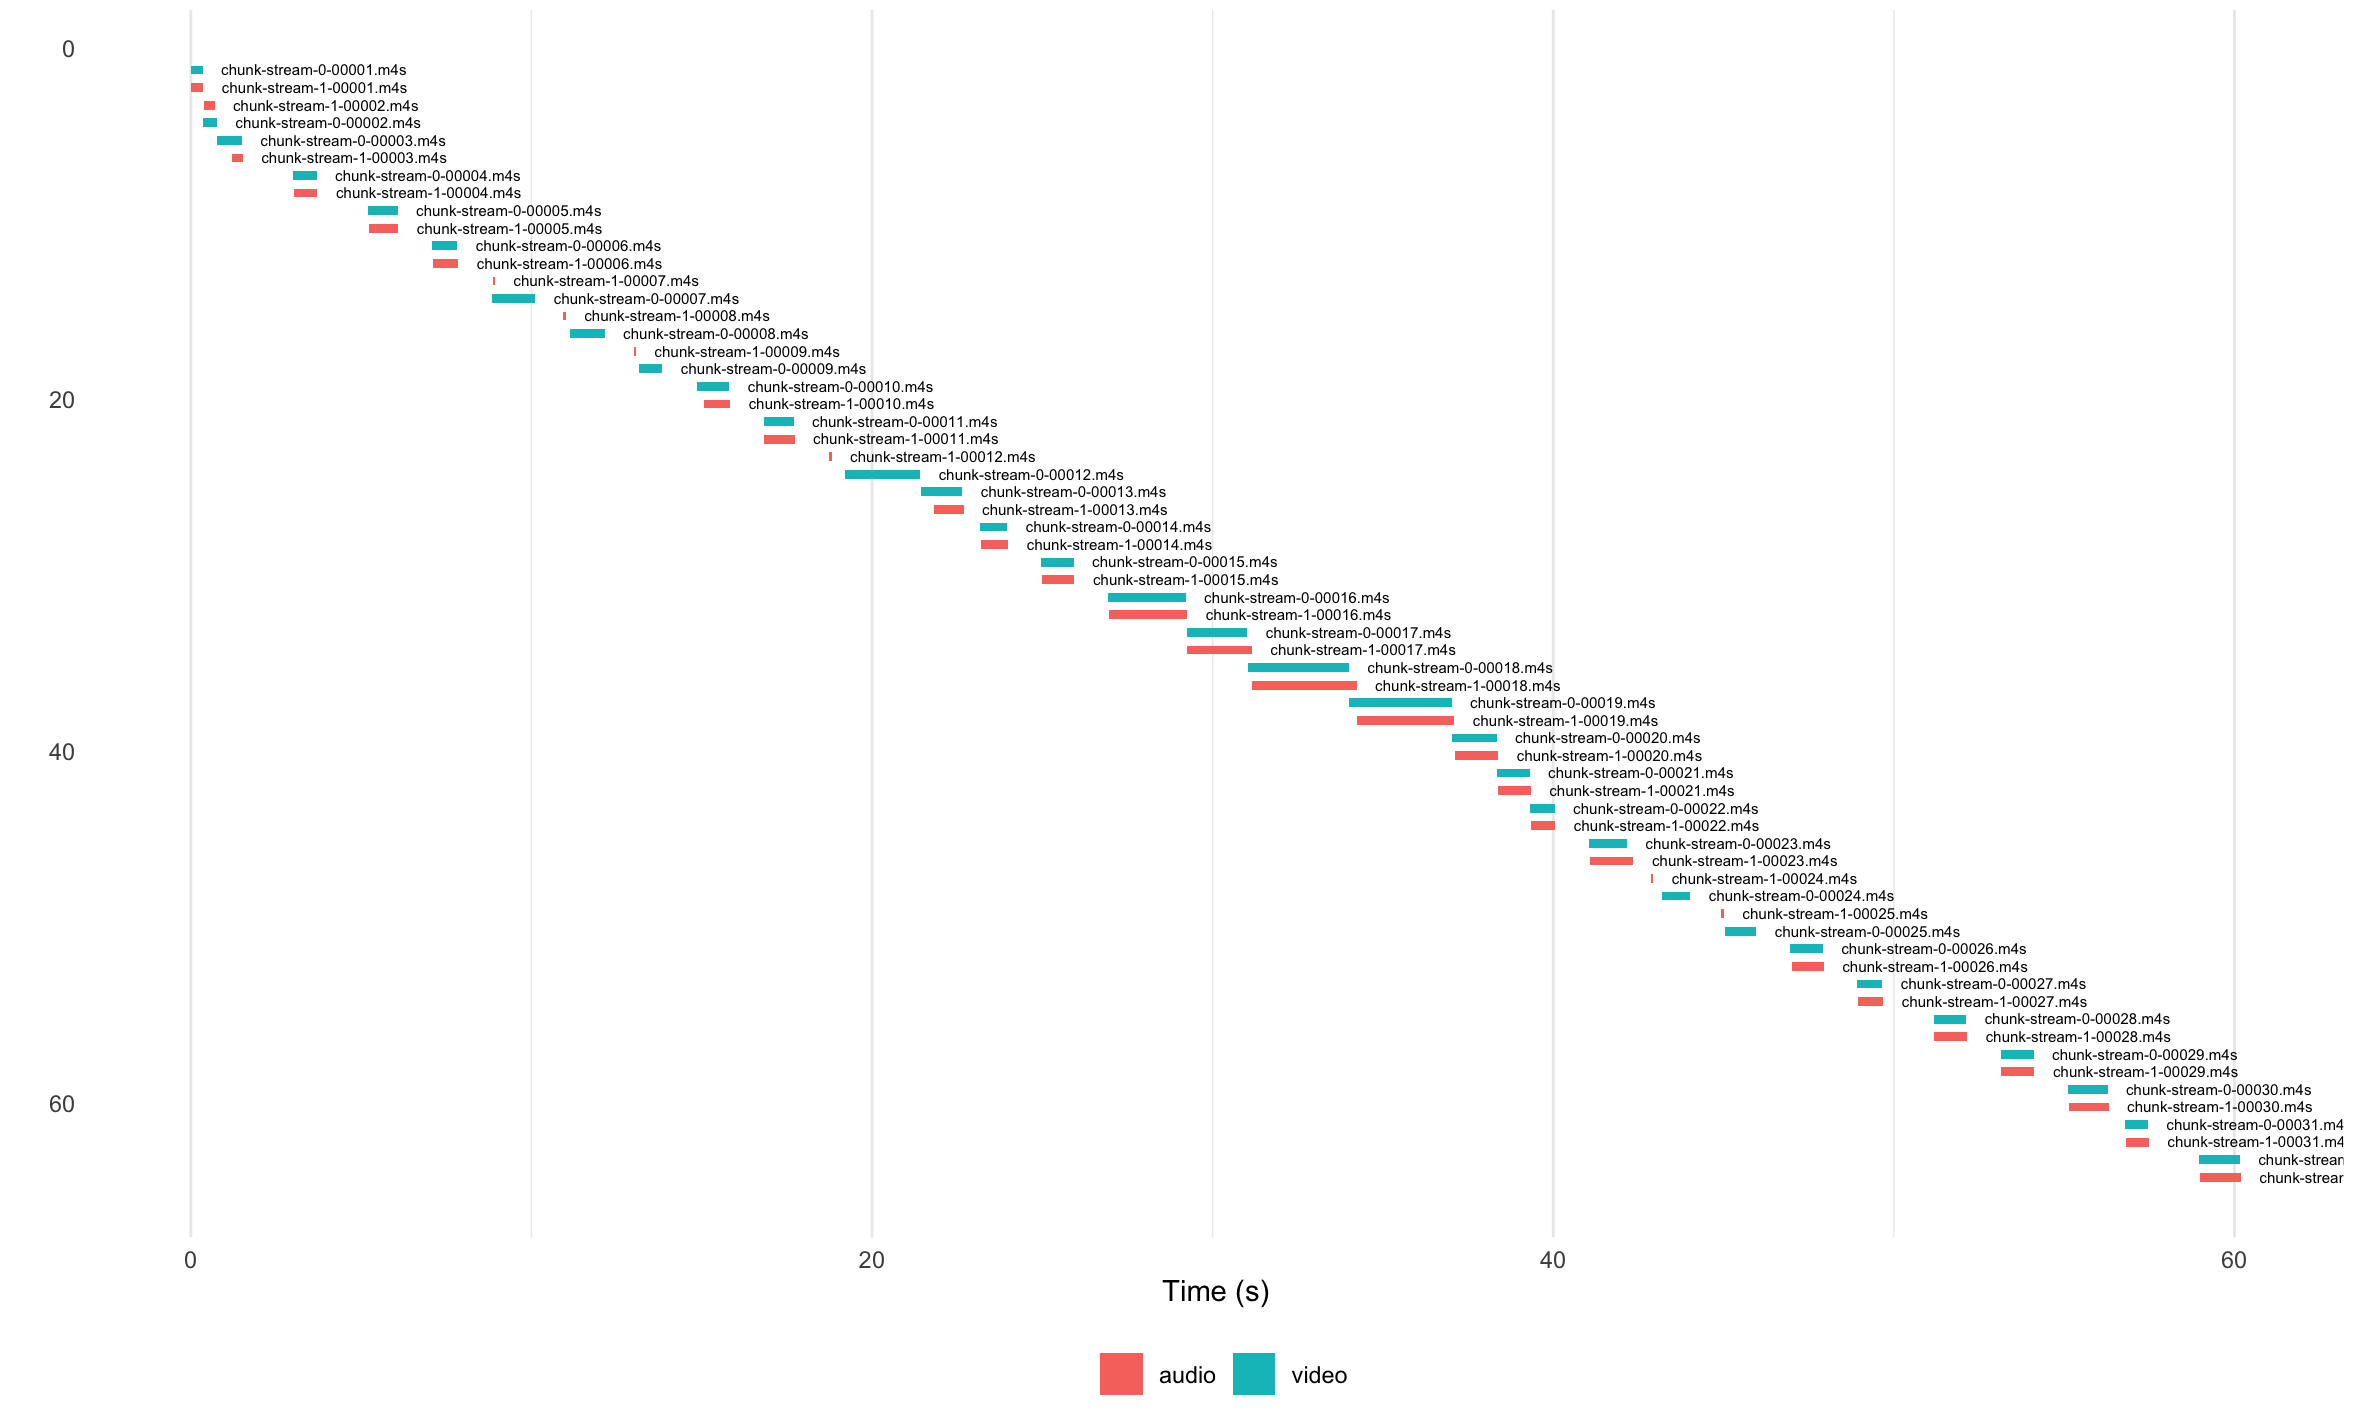
\includegraphics[width=0.9\textwidth]{res/eval_nonabr_lte_h3_waterfall.png}
    \caption{Waterfall diagram for DASH with the \texttt{lte} network pattern over HTTP/3.}
    \label{fig:eval_nonabr_lte_h3_waterfall}
\end{figure}

This behavior hints at a suboptimal scheduling strategy of HTTP requests over the QUIC connection, so we decided to investigate. We used the \textbf{NetLog dump} feature of Chromium (Section \ref{sec:bg/http3/tools}) to generate an export of network traffic, which also contains detailed information about QUIC connections and streams. We then analyzed the dump file with \texttt{qvis}.

One of the visualization tools provided by \texttt{qvis} is the multiplexing view, where the multiplexing of the streams at the QUIC level is represented both as a flow/timeline and as a waterfall (Figure \ref{fig:eval_noabr_qvis1}). The flow representation shows the sequence of QUIC packets that the client received. Each packet is colored with a different color depending on the stream to which it belongs. The waterfall view shows the same data as a waterfall chart, where each stream has its own row, and the horizontal segments represent the time intervals in which the stream was actively being transferred.

In our case, what we can clearly see in the multiplexing diagrams, especially in the waterfall, is that the streams are transmitted almost sequentially. In fact, there is almost no preemption, and most streams get to use the entire channel for transmission until all data is received.

\begin{figure}[h]
    \centering
    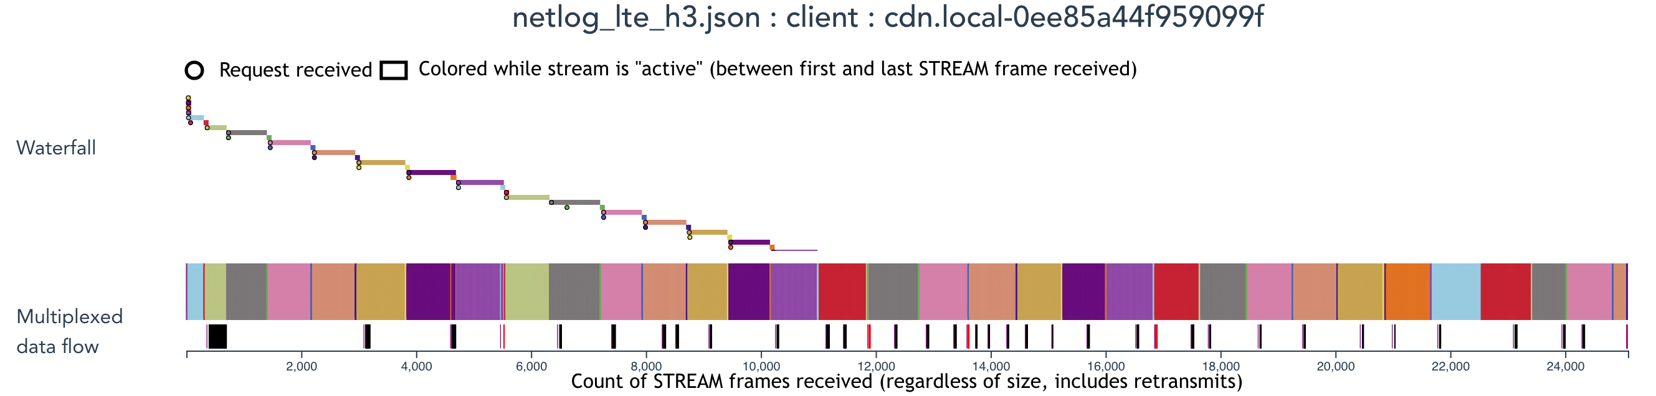
\includegraphics[width=0.9\textwidth]{res/eval_nonabr_qvis1.png}
    \caption{\texttt{qvis} multiplexing diagrams for the MPEG-DASH over HTTP/3 experiment.}
    \label{fig:eval_noabr_qvis1}
\end{figure}

However, an interesting fact to observe is that the data flow is not entirely sequential. As Figure \ref{fig:eval_noabr_qvis2} shows, there is a recurring pattern of streams/requests that start and are immediately suspended to give bandwidth to another stream on the QUIC connection.

This behavior explains what we were seeing in the segments requests waterfall in Figure \ref{fig:eval_nonabr_lte_h3_waterfall}. Requests for audio and video segments often start at the same time; however, the transfer of the audio segment is almost immediately preempted to give priority to the video segment. The audio segment transfer is then completed after the video segment is completely downloaded.

This behavior is not ideal, because an audio segment is always much smaller than a video segment and could therefore benefit from being received by the client earlier, as we will see in the next section. The next section will also compare how this same setup performs with HTTP/2 and HTTP/1.1, showing that the scheduling scheme that was observed seems to be specific to HTTP/3, or at least to the HTTP/3 implementation that we are relying on in this testbed.

The takeaway result of this analysis is that \textbf{we cannot rely on HTTP/3 implementations to always know the best strategy for request prioritization}. Instead, it is also the client/browser's responsibility to implement optimizations so that the prioritization strategy is meaningful.

The prioritization strategy could derive from browser heuristics that are applied globally for all websites, as we mentioned in Section \ref{sec:bg/http2}, but it could also be explicitly requested by developers with the use of priorities, as we explained in Section \ref{sec:eval/browsers/priorities}.

\begin{figure}[h]
    \centering
    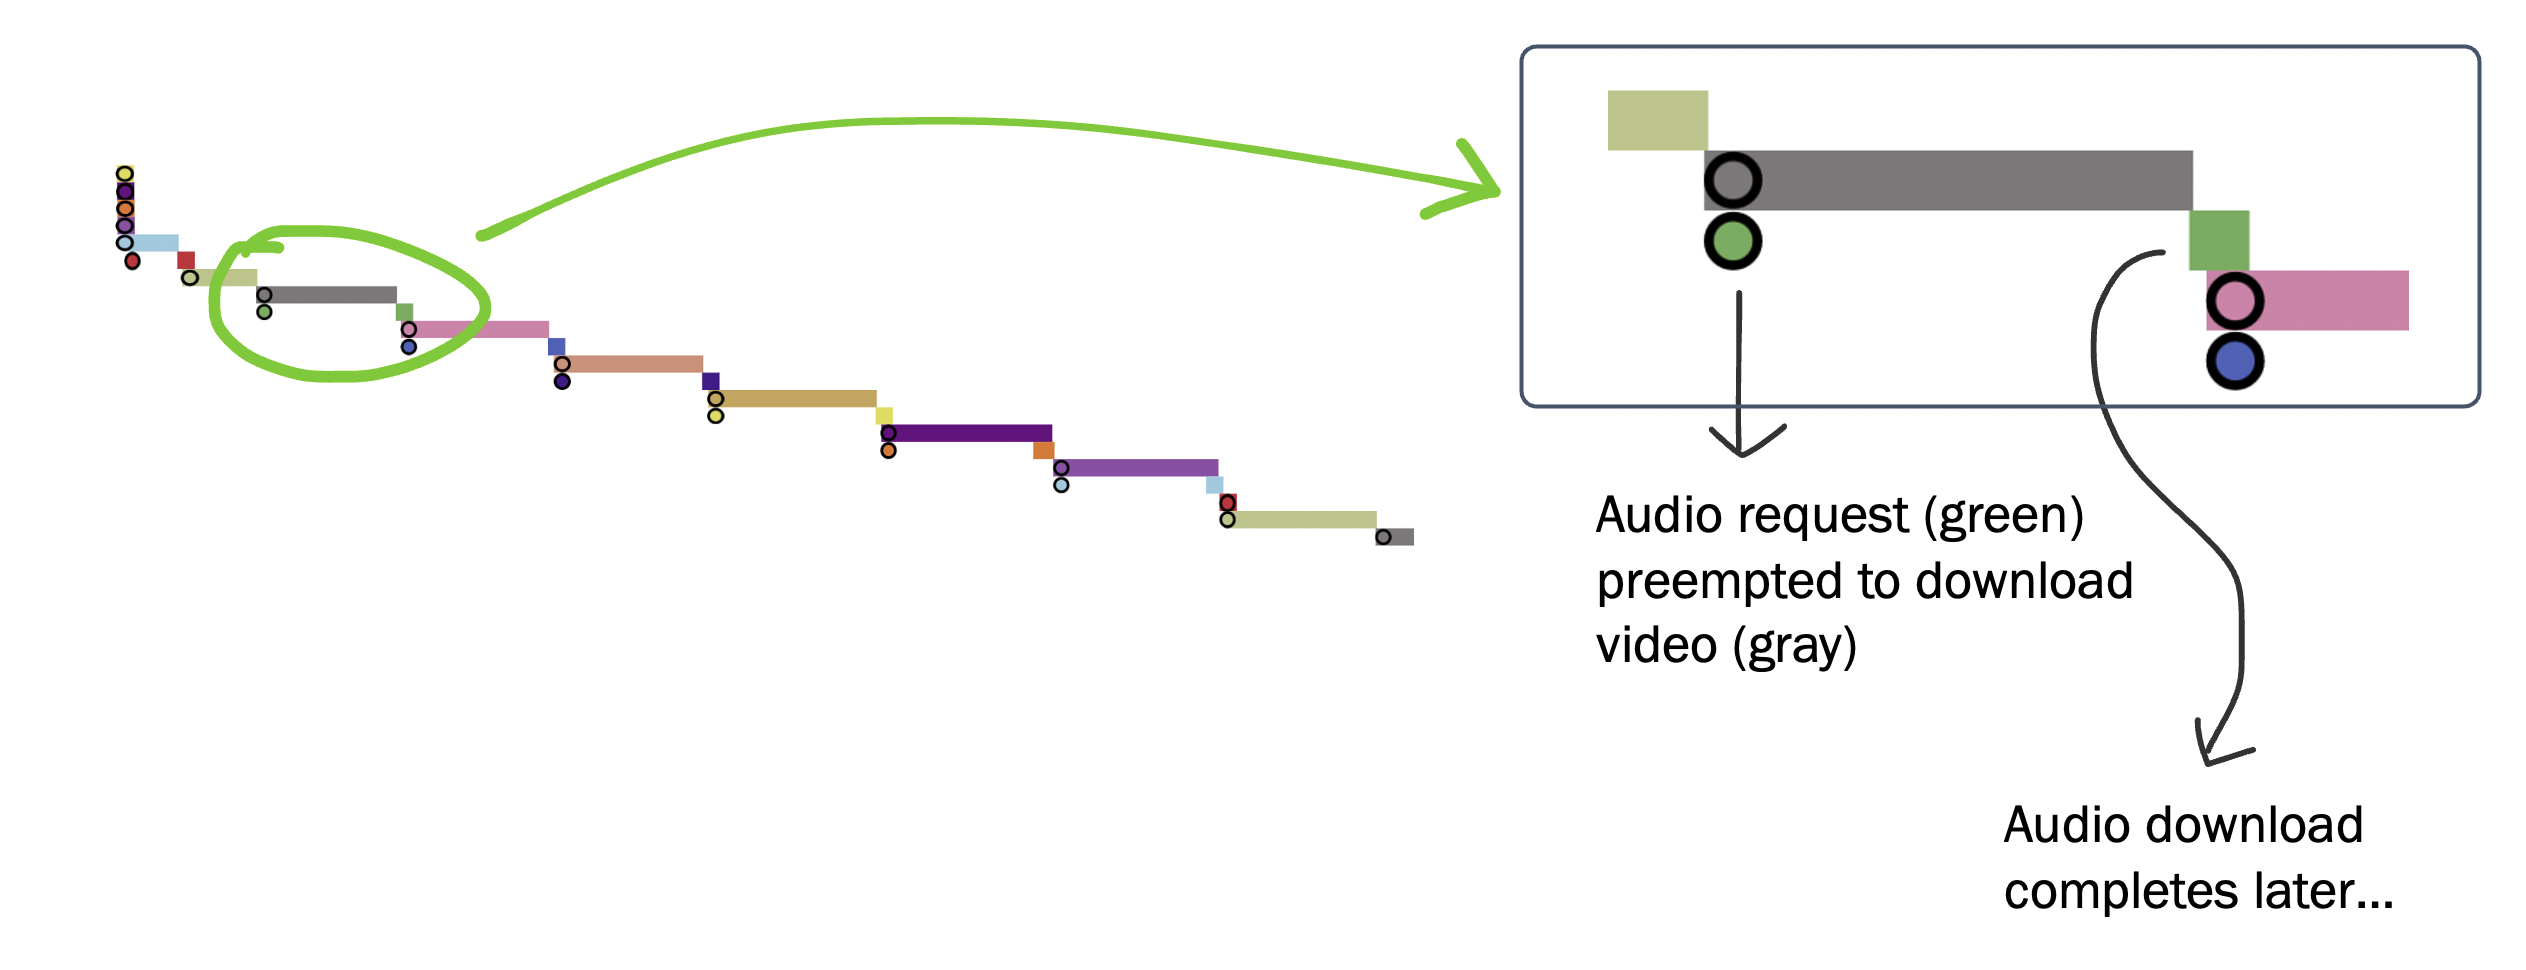
\includegraphics[width=0.9\textwidth]{res/eval_nonabr_qvis2.png}
    \caption{\texttt{qvis} waterfall diagram showing unexpected prioritization of video segments requests over audio with HTTP/3.}
    \label{fig:eval_noabr_qvis2}
\end{figure}

\subsection{Comparison across HTTP versions}
\label{sec:eval/non-abr/http-versions}

As we have seen, the emulation over HTTP/3 shows that priorities are not consistent, even in the same run. We will now see how HTTP/2 and HTTP/1.1 behave and then compare the results.

Let us start from \textbf{HTTP/2}. Figure \ref{fig:eval_nonabr_lte_h2_buffer} shows the buffer health plot for an experiment execution based on HTTP/2. The rest of the settings remained the same. As we can easily see, the behavior is quite different from HTTP/3. First, the audio buffer is always larger than the video. This means that the audio segments are consistently loaded before the video buffer. The waterfall in Figure \ref{fig:eval_nonabr_lte_h2_waterfall} confirms that this is because the audio segments are loaded much faster, as we would expect, and the loading of the video segments does not delay the audio. This behavior probably derives from a different prioritization strategy, implemented by the browser or driven by the HTTP/2 server implementation.

The other thing that we can observe is that there are no playback stalls, apart from the initial loading, even if the video buffer is almost empty for several seconds in the middle of the emulation. This behavior derives from the fact that the browser is capable of playing the audio data even if the video is not available, for up to 3 seconds. This particular \textbf{buffer underflow behavior} is specific to Chromium and is officially documented.\footnote{\url{https://www.chromium.org/audio-video/\#how-the-does-buffering-work}} Obviously, it can only work when audio and video data is appended to the MSE \texttt{SourceBuffer} independently; therefore, in practice, it can only happen when using unmuxed video and audio tracks, as is in our case.

Although Chromium's underflow behavior might not be the expected experience when streaming on-demand content, since it has the effect of not rendering the video for a few seconds, it seems instead to be particularly suitable for live streaming. In fact, in this way \textbf{short time intervals where video data is not available do not cause a stall}, and, therefore, \textbf{do not increase the latency of the live stream}. While the video is frozen due to a slow loading segment, \textbf{the audio will continue to play}.

\begin{figure}[h]
	\centering
	
	\begin{subfigure}[t]{0.45\textwidth}
		\centering
		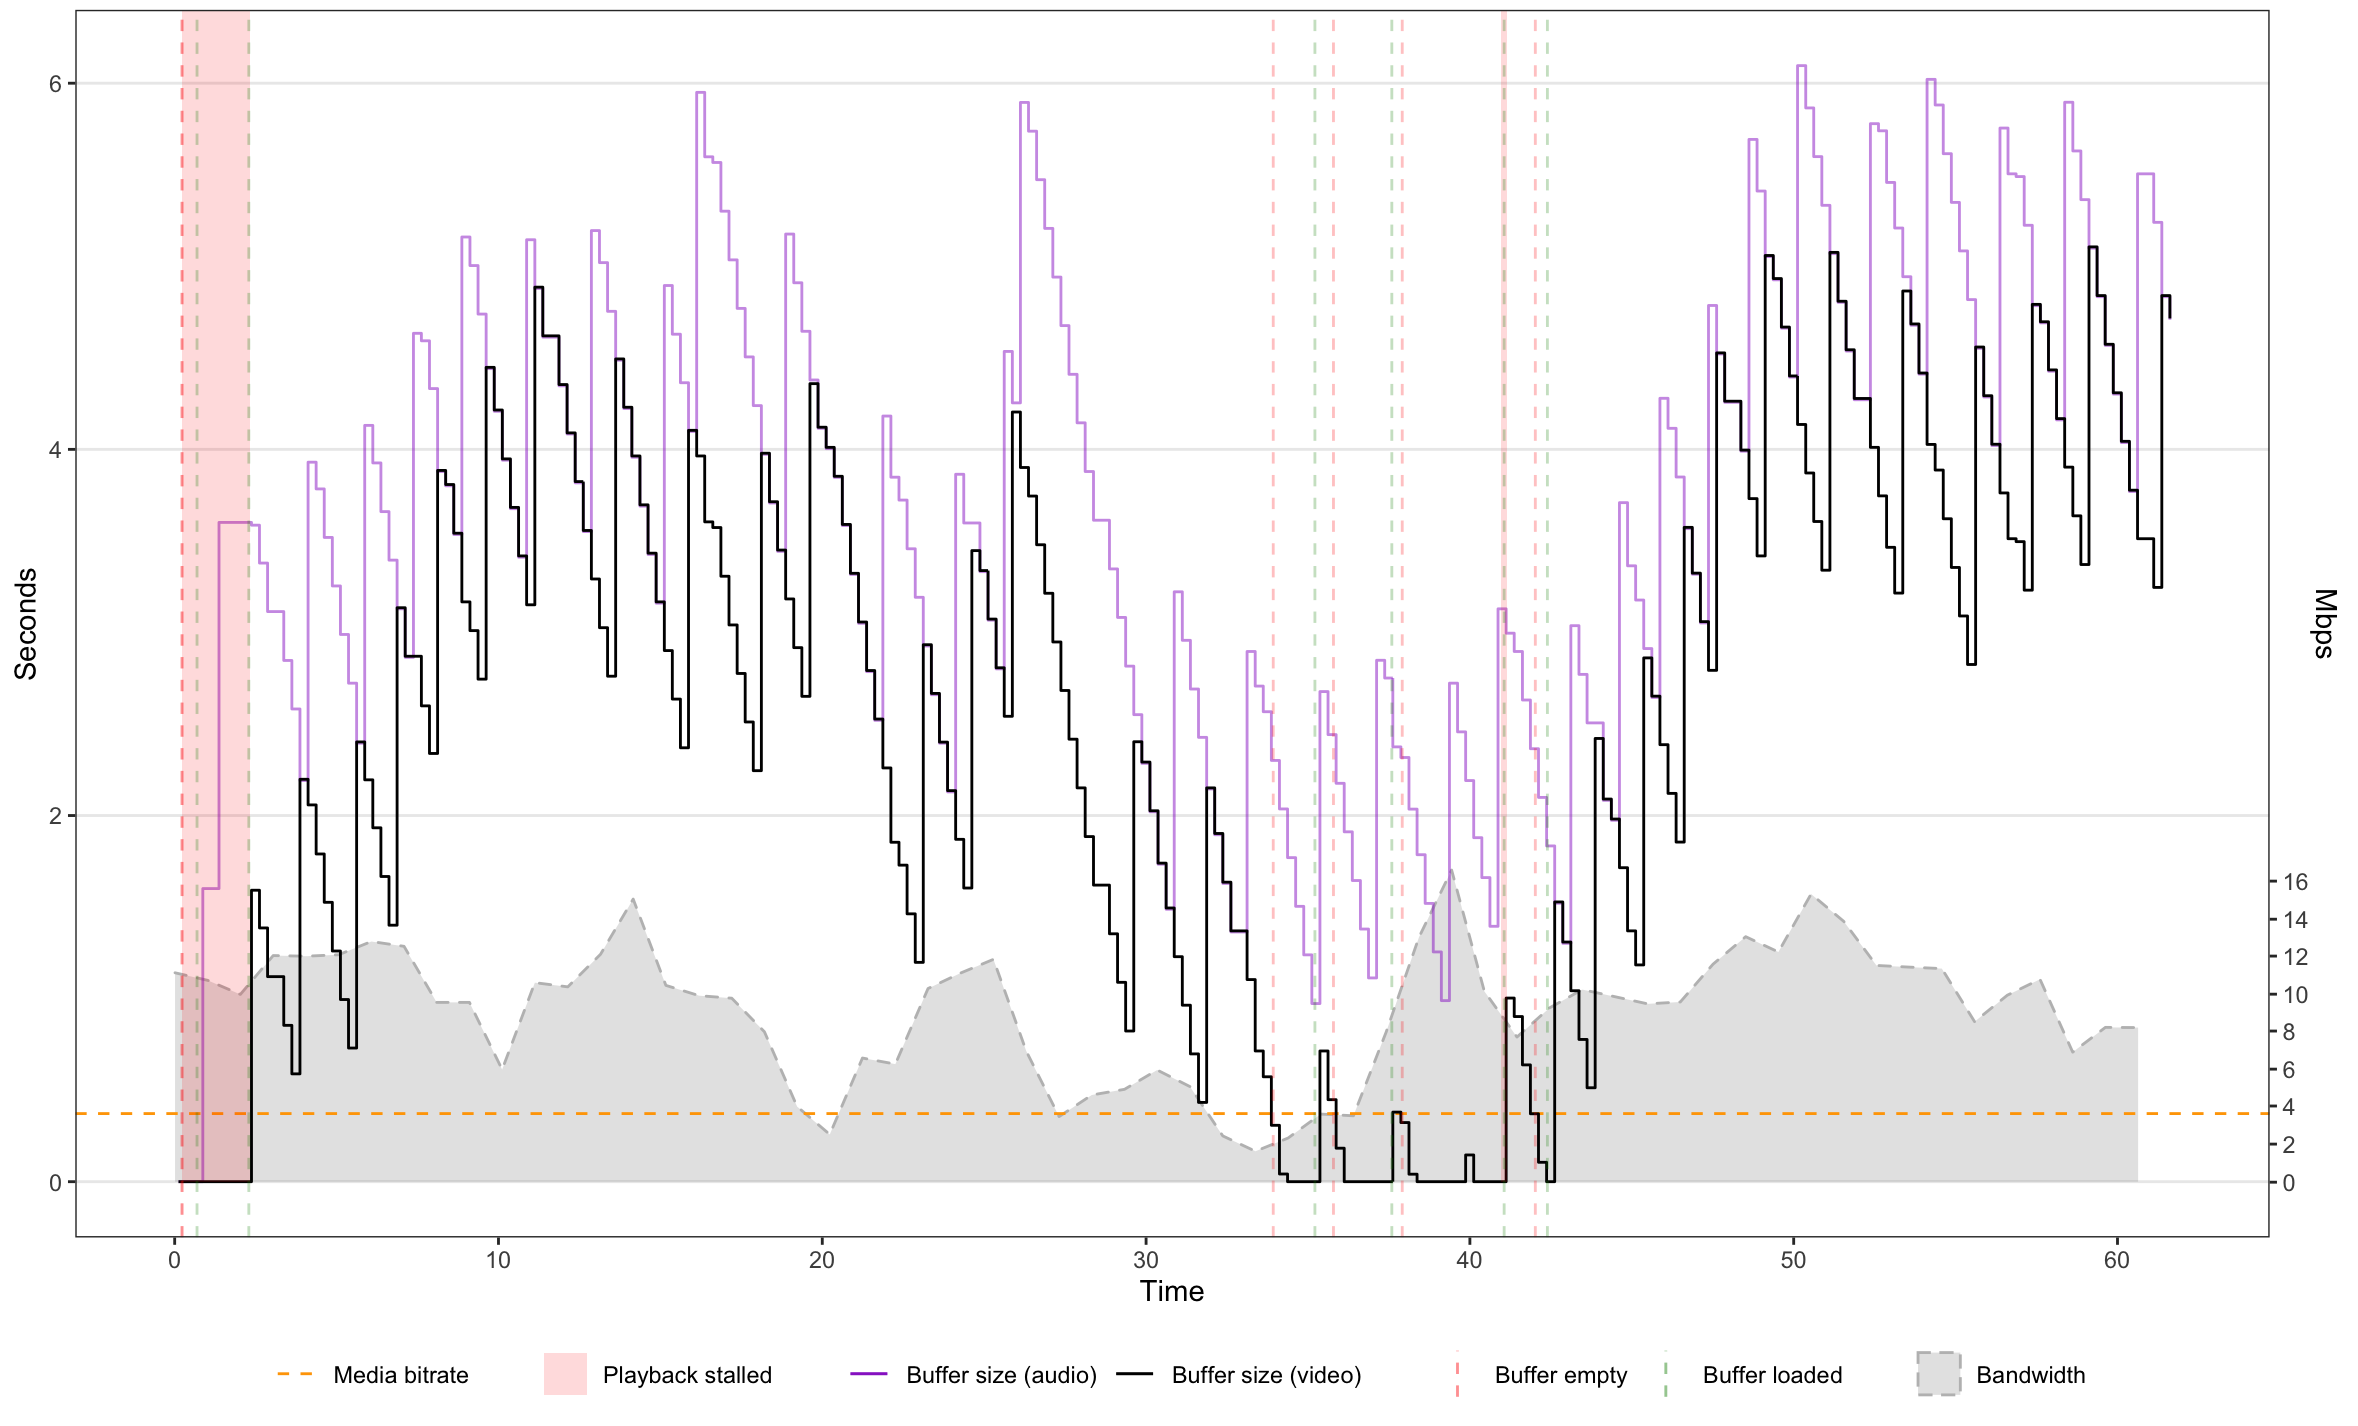
\includegraphics[width=\textwidth]{res/eval_nonabr_lte_h2.png}
		\caption{Buffer health plot.}
		\label{fig:eval_nonabr_lte_h2_buffer}
	\end{subfigure}%
	~ 
	\begin{subfigure}[t]{0.45\textwidth}
		\centering
		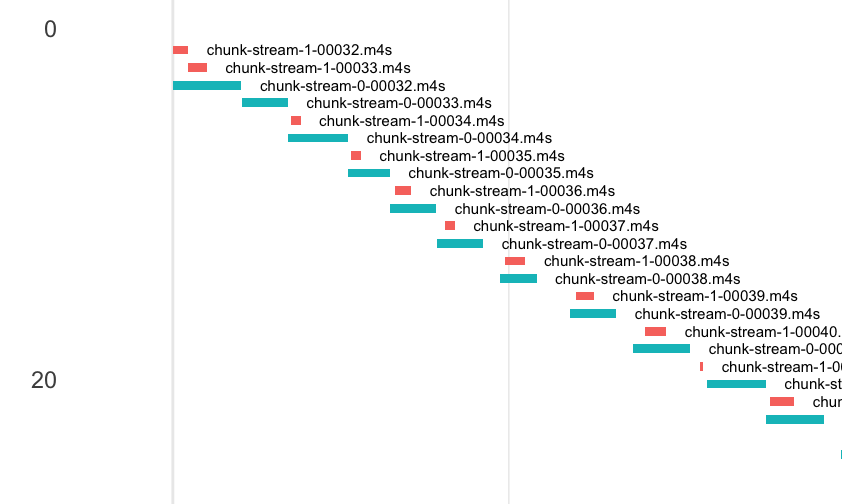
\includegraphics[width=\textwidth]{res/eval_nonabr_lte_h2_waterfall.png}
		\caption{Waterfall diagram.}
		\label{fig:eval_nonabr_lte_h2_waterfall}
	\end{subfigure}
	
	\caption{DASH experiment over HTTP/2 with the \texttt{lte} network pattern.}
	\label{fig:eval_nonabr_lte_h2}
\end{figure}

Moving on to \textbf{HTTP/1.1}, the behavior that we observed is somewhat similar to HTTP/2. As Figure \ref{fig:eval_nonabr_lte_h1_buffer} shows, the audio buffer is virtually always longer than the video buffer. One thing to note is that there is a playback stall at about 38 seconds, even if the audio buffer contains several seconds of data. This is due to the limitations of the underflow tolerance we have just introduced: Chromium only allows the video track to have missing data for about 3 seconds, after which the playback will stall. We will address this limitation in Chapter \ref{cha:improvements}.

The waterfall diagram for HTTP/1.1, shown in \ref{fig:eval_nonabr_lte_h1_waterfall}, is perhaps even more interesting. It shows that the download of the audio segments, represented in red, is consistently completed in a very short amount of time. Intuitively, the explanation for this phenomenon is that HTTP/1.1 can use multiple independent TCP connections, not performing multiplexing at all. In this way, requests can be distributed among the connections and benefit from a "dedicated" transmission channel.

\begin{figure}[h]
	\centering
	
	\begin{subfigure}[t]{0.45\textwidth}
		\centering
		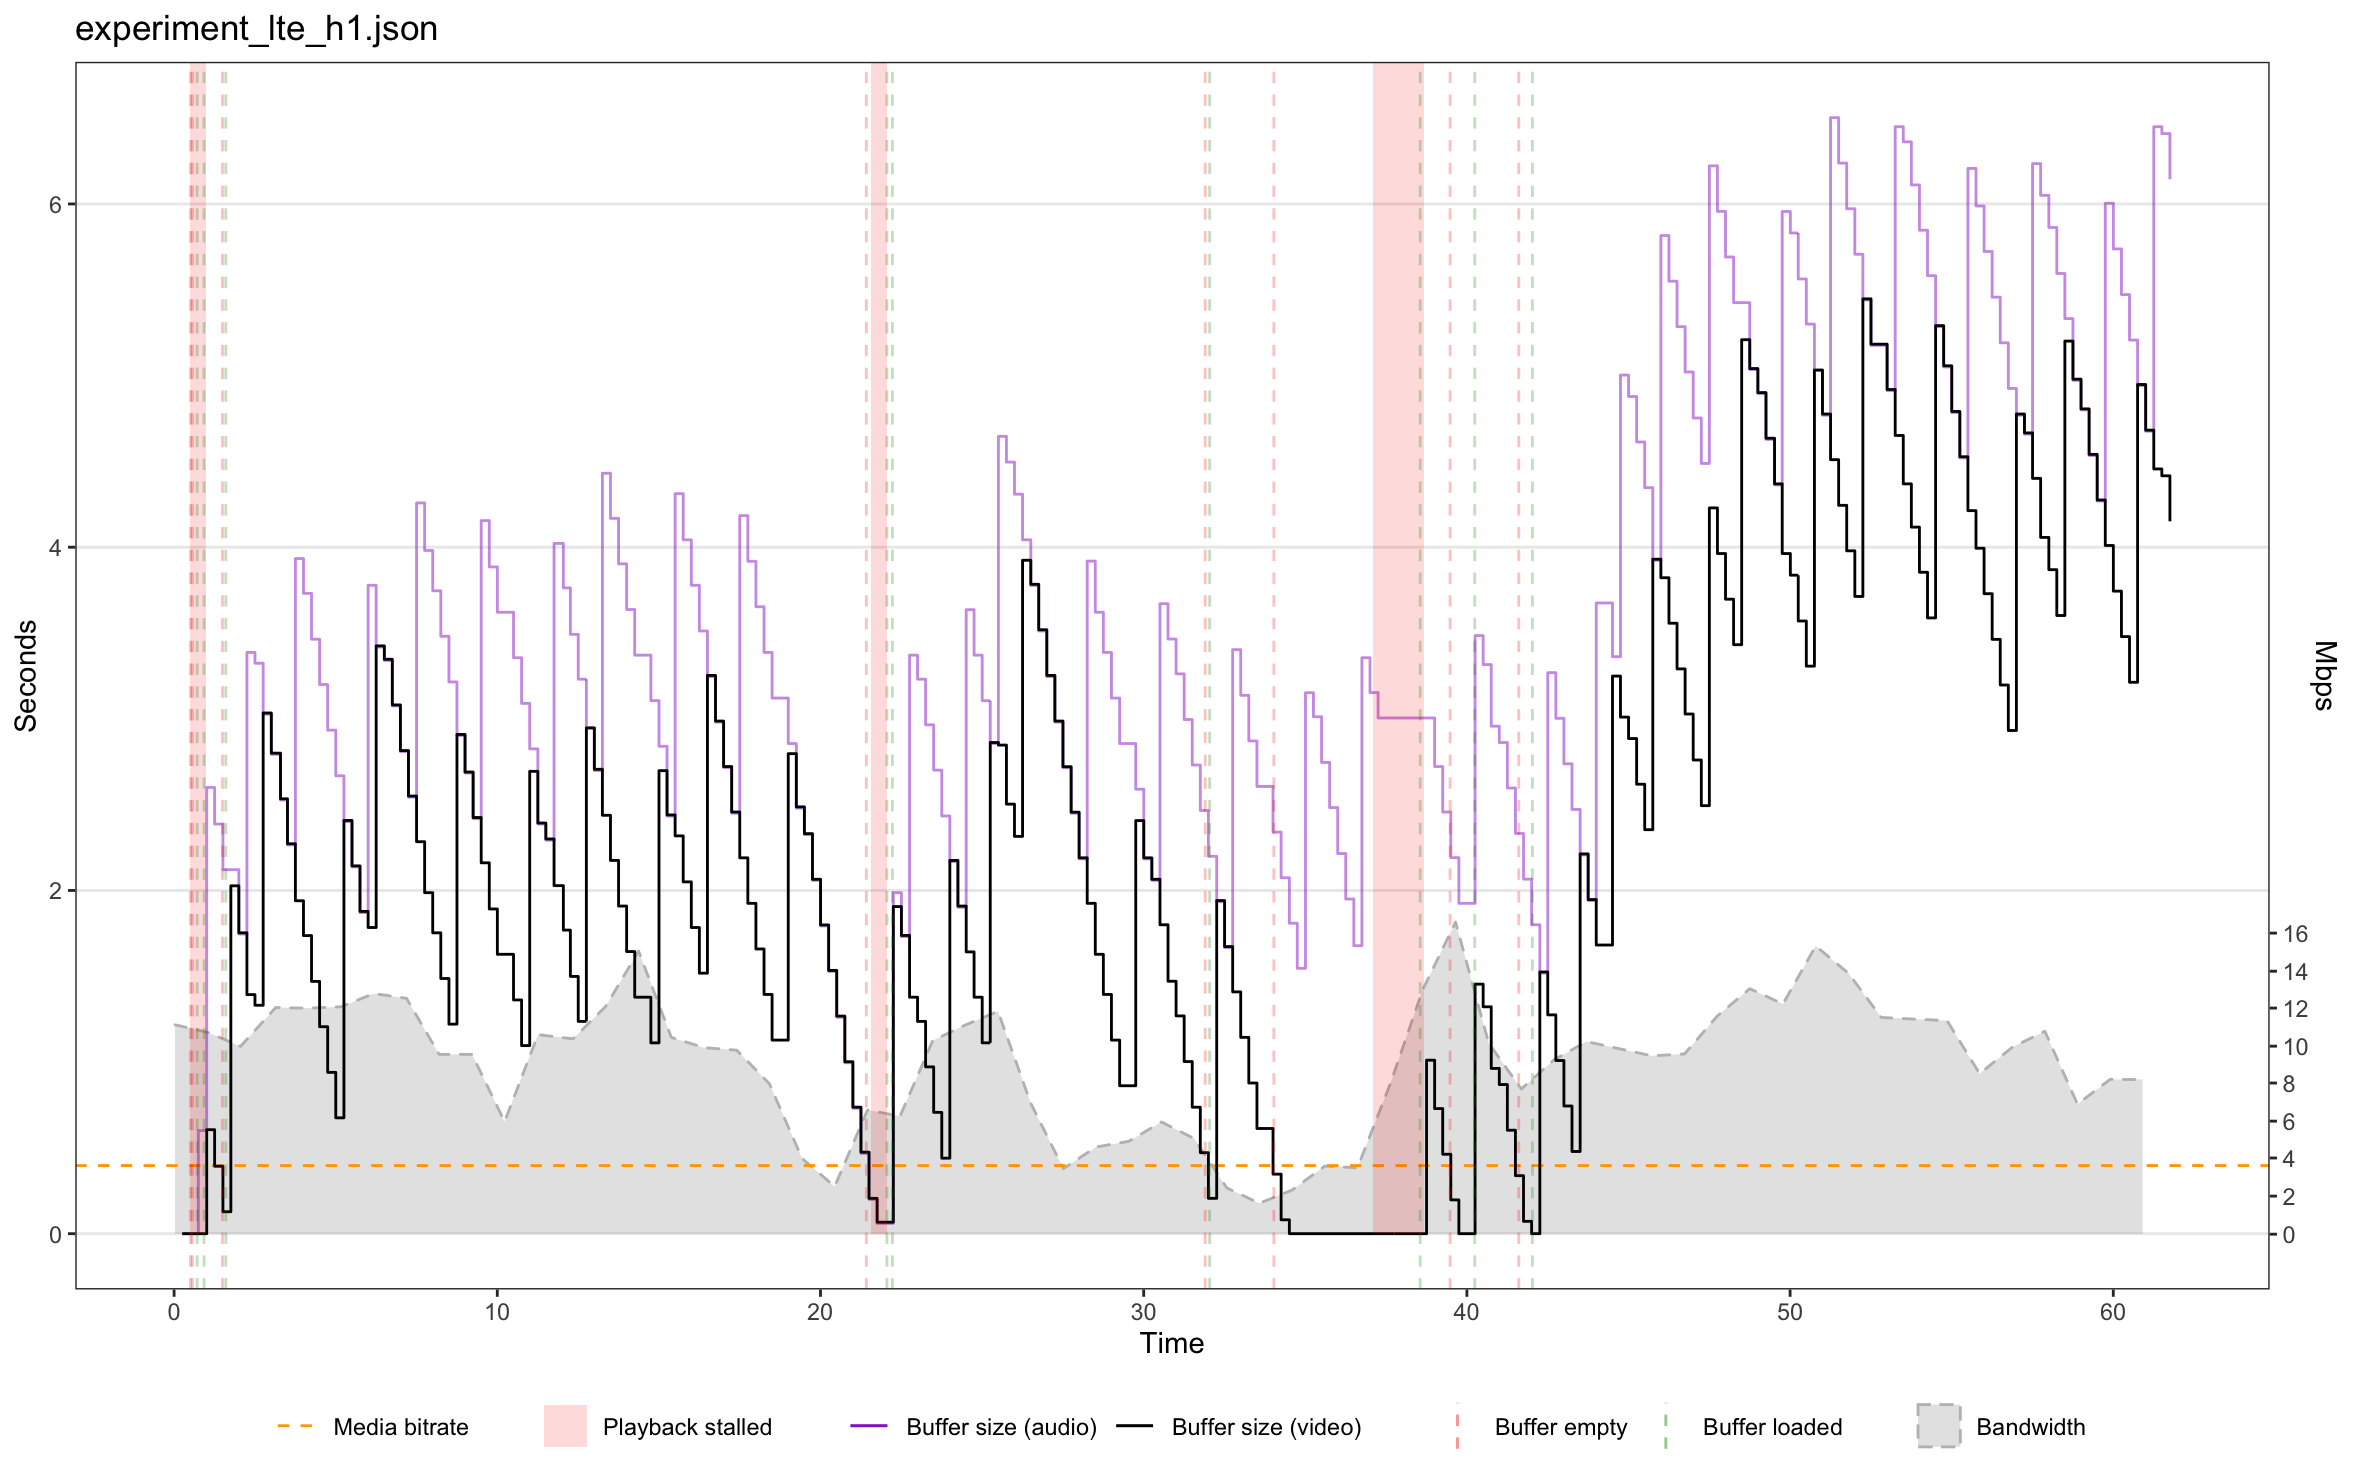
\includegraphics[width=\textwidth]{res/eval_nonabr_lte_h1.png}
		\caption{Buffer health plot.}
		\label{fig:eval_nonabr_lte_h1_buffer}
	\end{subfigure}%
	~ 
	\begin{subfigure}[t]{0.45\textwidth}
		\centering
		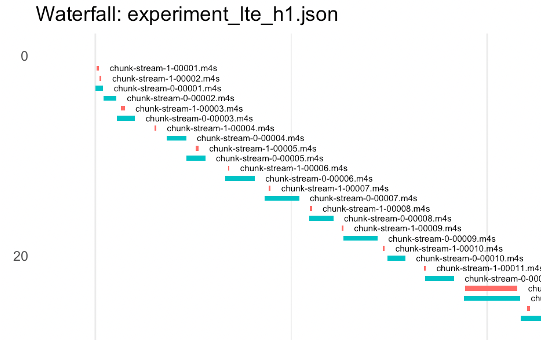
\includegraphics[width=\textwidth]{res/eval_nonabr_lte_h1_waterfall.png}
		\caption{Waterfall diagram.}
		\label{fig:eval_nonabr_lte_h1_waterfall}
	\end{subfigure}
	
	\caption{DASH experiment over HTTP/1 with the \texttt{lte} network pattern.}
	\label{fig:eval_nonabr_lte_h1}
\end{figure}

These results are surprising. We are seeing that HTTP/2 and HTTP/1.1 appear to offer better scheduling of requests. Incidentally, this also translates into a live streaming experience that has fewer "hard" stalls and where the latency does not increase.

\subsection{The need for adaptive bitrate streaming}
\label{sec:eval/non-abr/adaptive}

The experiments mentioned above were conducted with the \texttt{lte} network pattern, where the network bandwidth is most of the time higher than the media bitrate. In the \texttt{hspa+} pattern, the situation is different: the bandwidth is just slightly above the media bitrate and often goes below it. This is pretty clear from Figure \ref{fig:eval_nonabr_hspa+_h3_buffer}, where there are many stalls in all situations where the bandwidth is not enough. The consequence is that the live latency increases during the playback stall periods, reaching 23 seconds as shown in Figure \ref{fig:eval_nonabr_hspa+_h3_waterfall}.

\begin{figure}[h]
	\centering
	
	\begin{subfigure}[t]{0.45\textwidth}
		\centering
		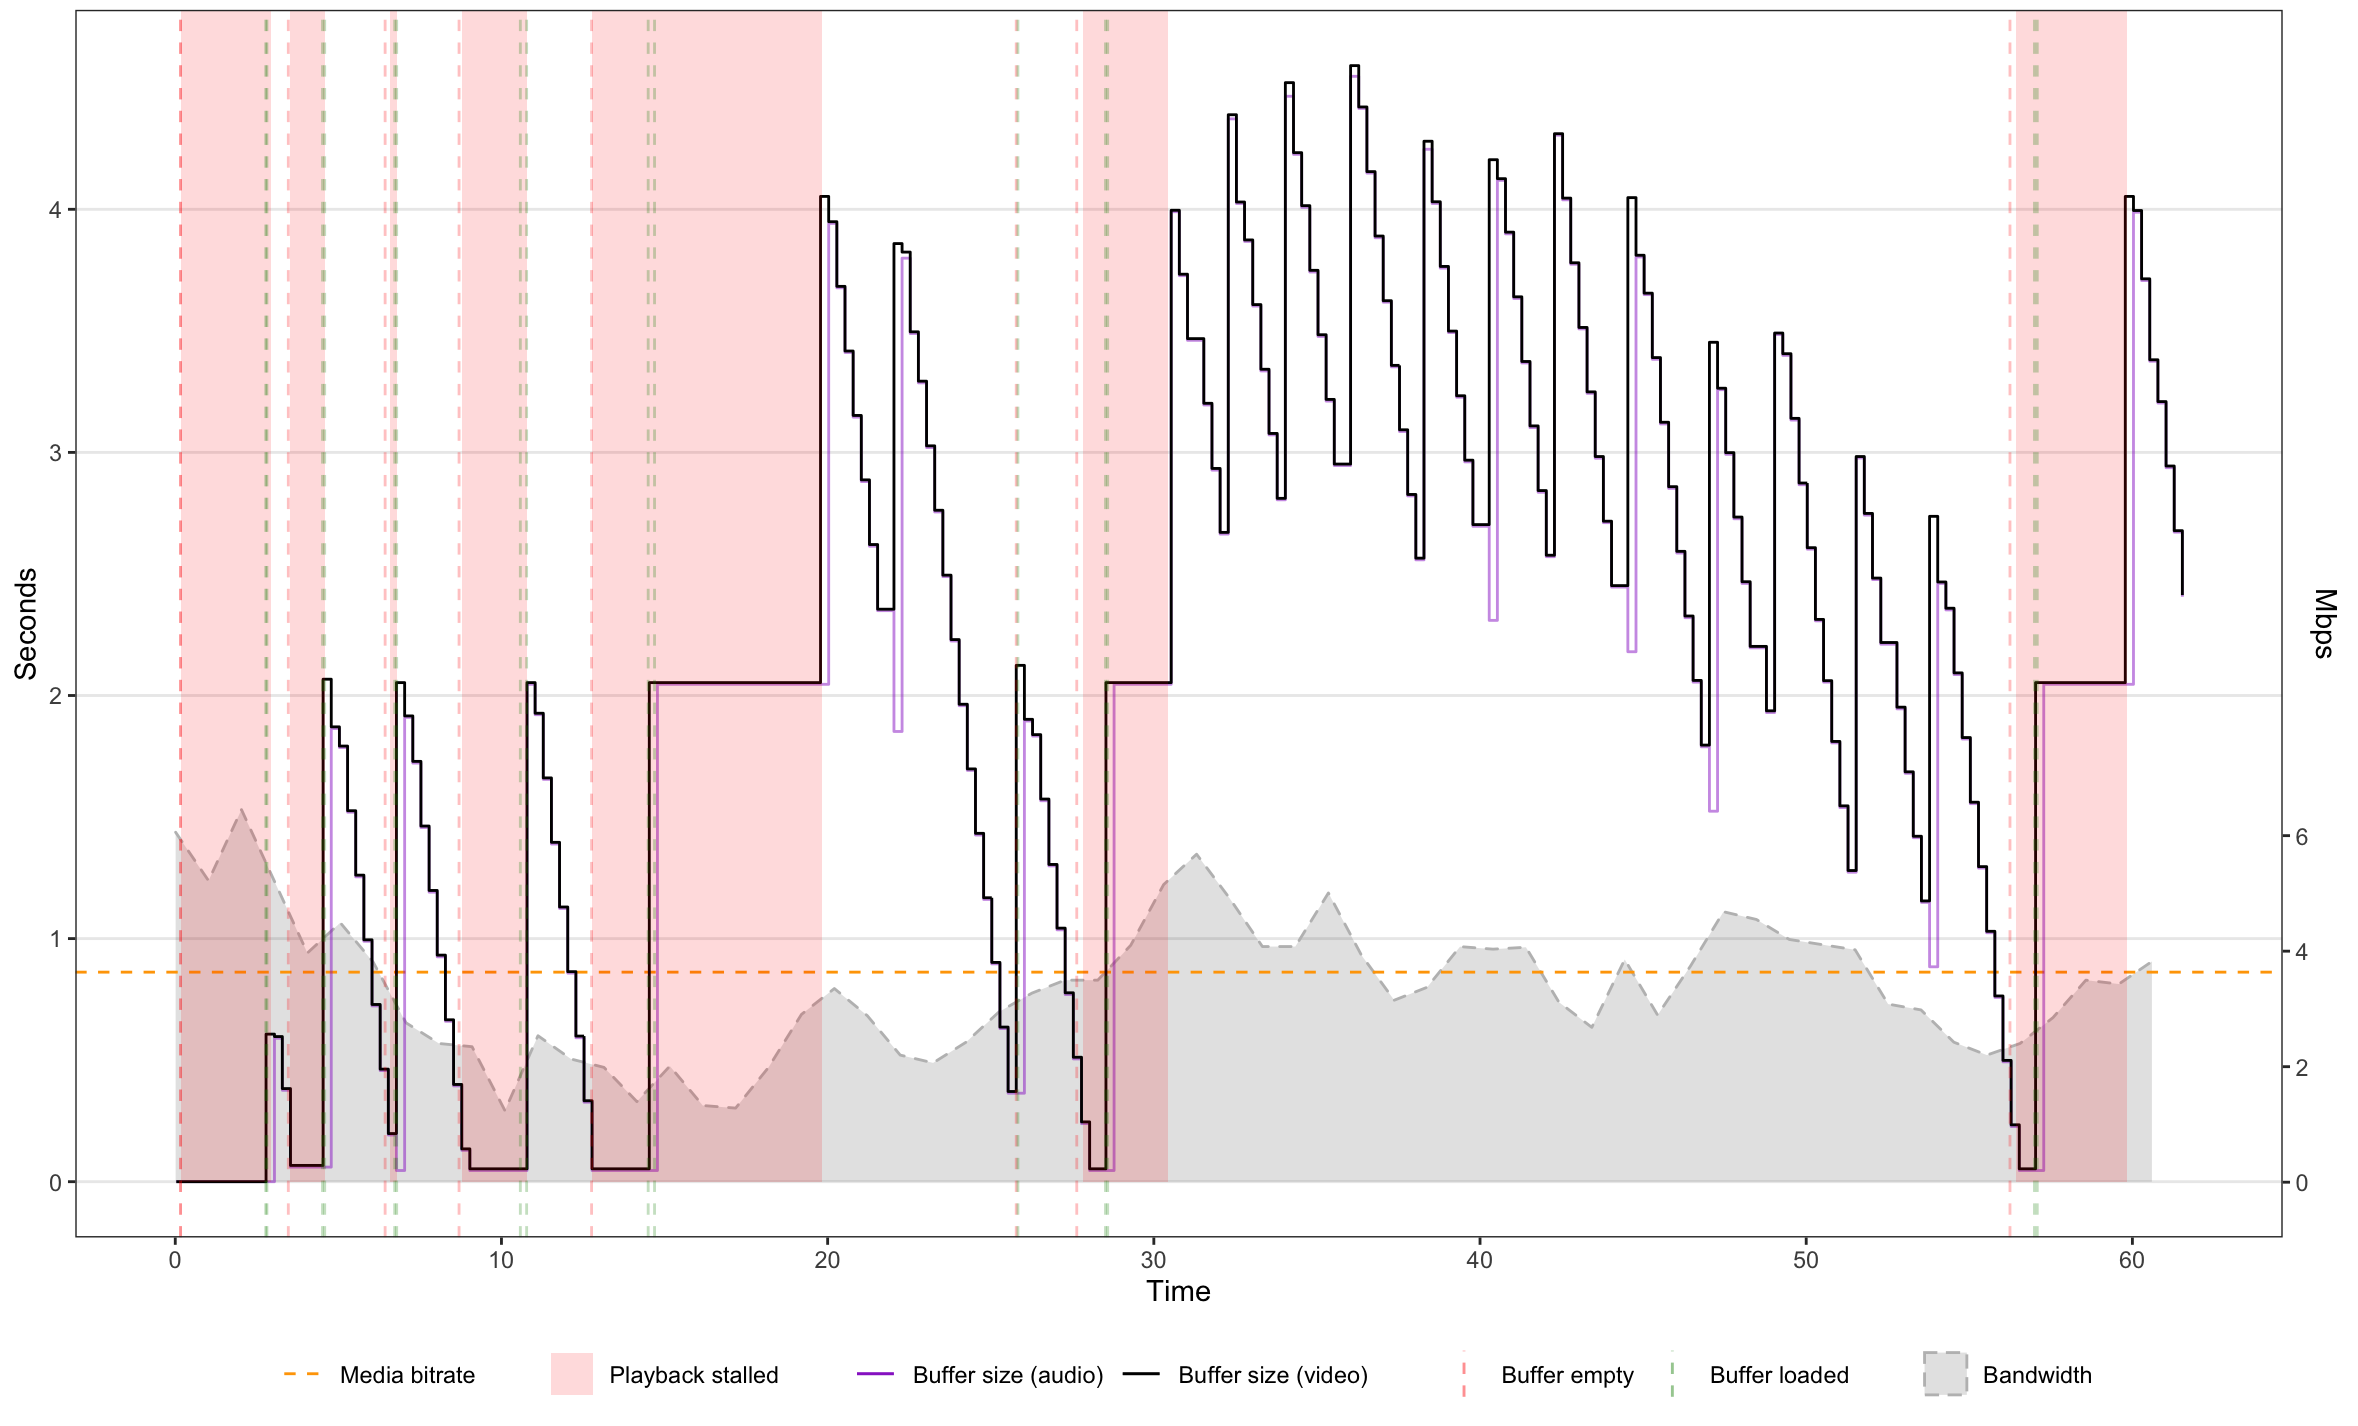
\includegraphics[width=\textwidth]{res/eval_nonabr_hspa+_h3.png}
		\caption{Buffer health plot.}
		\label{fig:eval_nonabr_hspa+_h3_buffer}
	\end{subfigure}%
	~ 
	\begin{subfigure}[t]{0.45\textwidth}
		\centering
		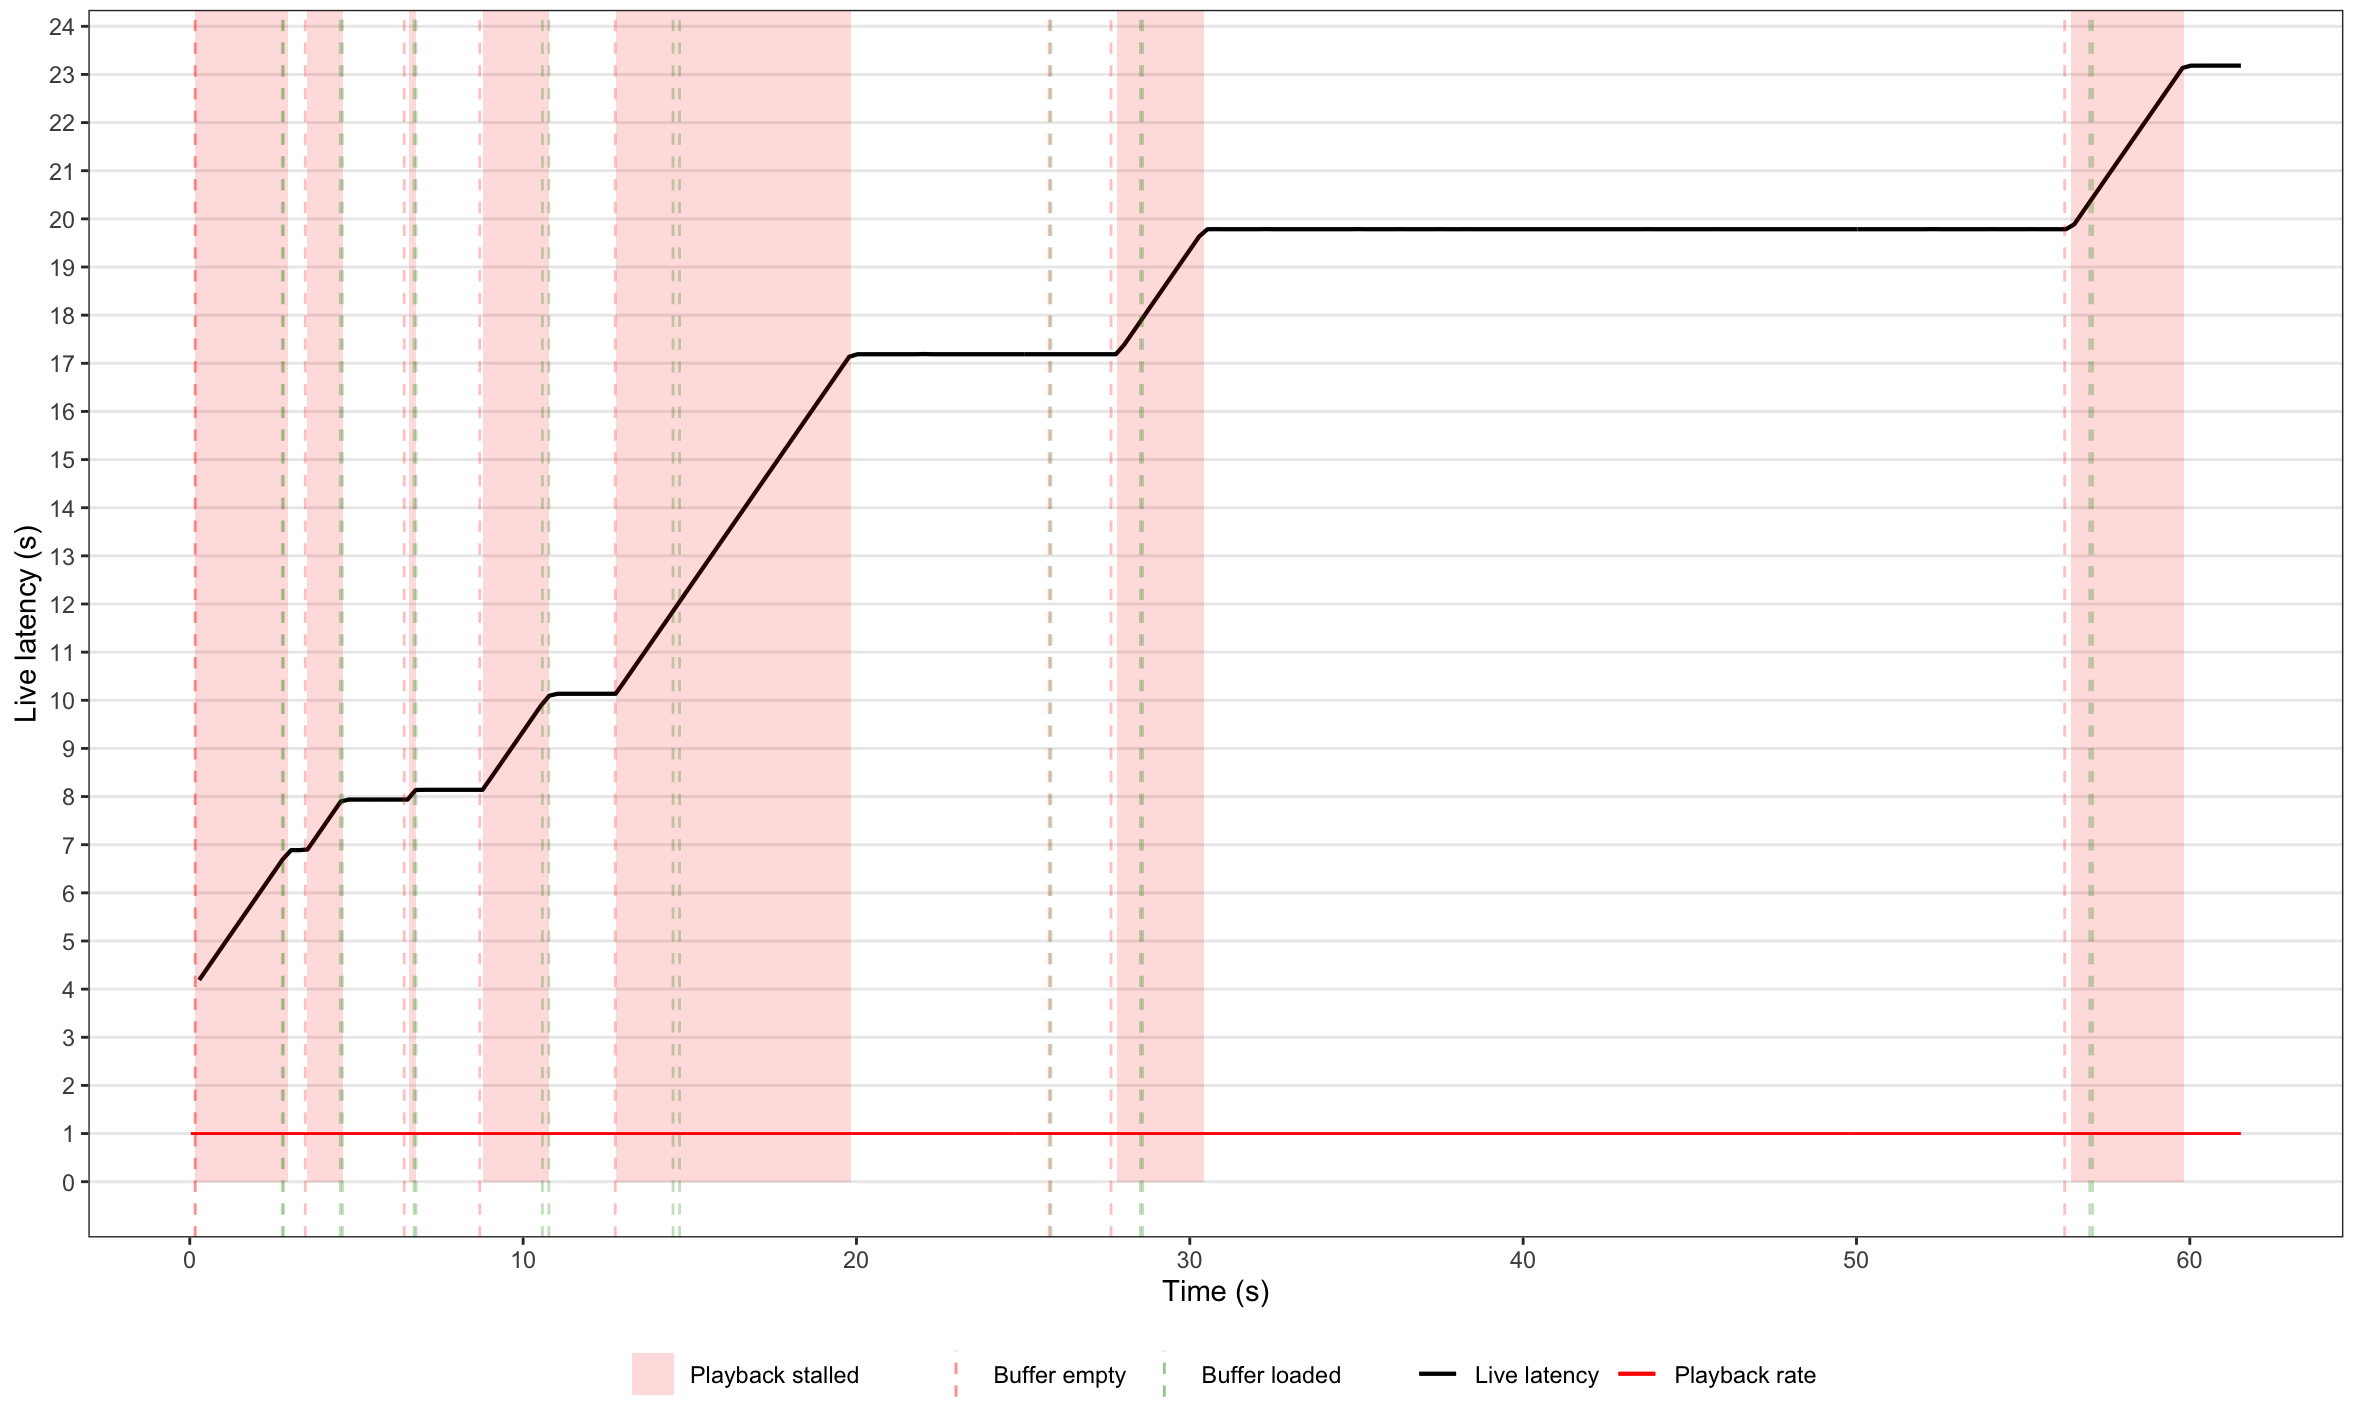
\includegraphics[width=\textwidth]{res/eval_nonabr_hspa+_h3_latency.png}
		\caption{Live latency plot.}
		\label{fig:eval_nonabr_hspa+_h3_waterfall}
	\end{subfigure}
	
	\caption{DASH experiment over HTTP/3 with the \texttt{hspa+} network pattern.}
	\label{fig:eval_nonabr_hspa+_h3}
\end{figure}

\textbf{Adaptive bitrate streaming} is needed for this reason: when the adaptation algorithm estimates that there is not enough bandwidth to continue the playback at the current bitrate, it will make the decision to switch to a lower bitrate. In the next sections, we will see how the system performs when adaptive bitrate streaming is enabled.

\section{Experiments and results in an ABR setup}
\label{sec:eval/abr}

The testbed that we introduced in Chapter \ref{cha:testbed} is already capable of running experiments on an adaptive live stream. In fact, if we do not specify the minimum bitrate in the experiment configuration, the playback will use ABR. We tested this setup with both \dashjs{} and \hlsjs{}.

\subsection{Suboptimal behavior of the default \dashjs{} configuration with live}
\label{sec:eval/abr/dashjs}

An experiment we ran involved using \dashjs{} with ABR enabled and on the \texttt{lte} network pattern. As a reminder, the bitrate ladder we are using in this experiment is made of four resolutions (720p, 540p, 360p, 270p) with video bitrates of 3.5 Mbps, 2.5 Mbps, 1.5 Mbps and 0.8 Mbps.

The buffer health plot in Figure \ref{fig:eval_abr_dashjs} shows that with this configuration buffer underflows and playback stalls are essentially eliminated, compared to Figure \ref{fig:eval_nonabr_lte_h3} (non-ABR case) where there were multiple stalls. This is due to the fact that the default configuration of \dashjs{} is relatively aggressive in downswitching the resolution/bitrate. Therefore, it is able to quickly react to the worsening network conditions at about 30 seconds, and lower the bitrate to 2.5 and then 1.5 Mbps. A similar result (not shown here) is obtained with the \texttt{hspa+} pattern.

\begin{figure}[h]
    \centering
    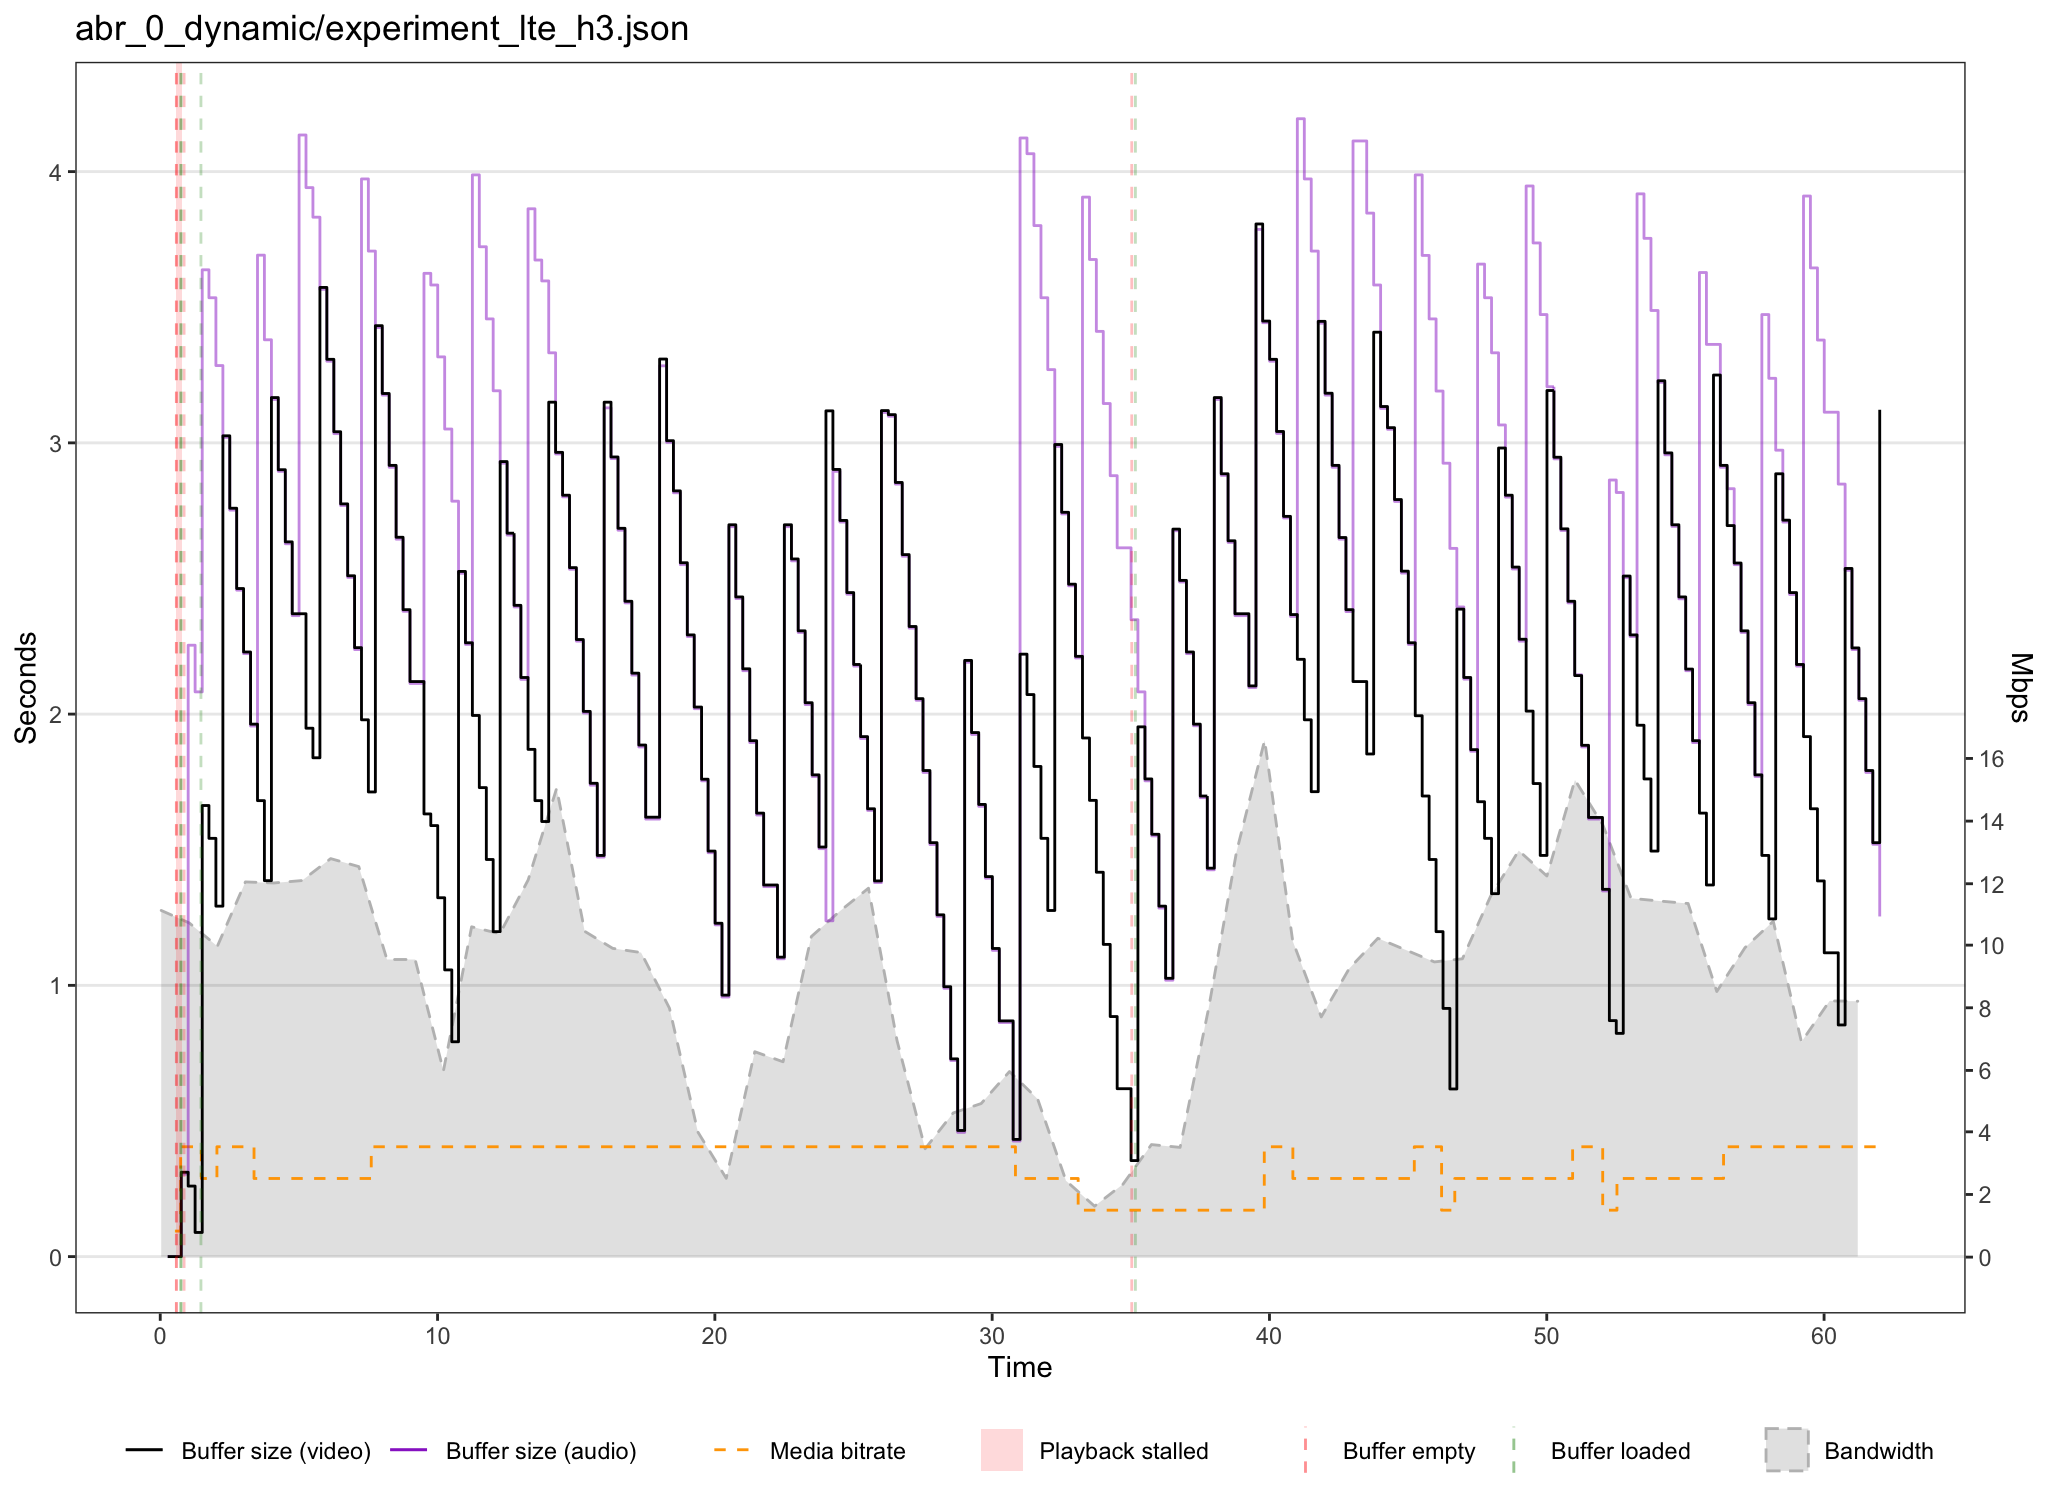
\includegraphics[width=0.9\textwidth]{res/eval_abr_dash_dynamic.png}
    \caption{Buffer health plot of an ABR DASH experiment with default configuration over HTTP/3 with the \texttt{lte} network pattern.}
    \label{fig:eval_abr_dashjs}
\end{figure}

There is, however, an evident disadvantage to this aggressive approach, which can be seen between second 40 and second 60 in the plot. The bandwidth is always above 8 Mbps in that interval of the experiment, and thus there should be more than enough bandwidth to keep the stream at the highest quality and bitrate (3.5 Mbps).

Instead, what we observe is that the adaptation algorithm keeps switching quality in a way that does not seem to make much sense. At second 40, the bitrate is raised to 3.5 Mbps but almost immediately switched down to 2.5 Mbps. The algorithm then tries to raise the bitrate again and immediately falls to 1.5 Mbps. This oscillating pattern is repeated a few times until the experiment is over.

We observed that this behavior is consistent between different runs of the same experiment and is therefore something that should be investigated.

\subsection{Other network patterns and experiments with \hlsjs{}}
\label{sec:eval/abr/hls}

To find a situation where the adaptation algorithm does not behave well and leads to playback stalls, we relied on new network patterns inspired by Twitch's dataset for low-latency scenarios, introduced in Section \ref{sec:testbed/network/patterns}. Specifically, for this analysis we will take into consideration the \texttt{spike} pattern, which contains an abrupt drop in bandwidth that lasts for a few seconds. The duration of the experiments based on this pattern is about 30 seconds.

At this point of the analysis, we also had a complete implementation of the integration with \hlsjs{} in the testbed, and therefore we ran the experiments with both \dashjs{} and \hlsjs{}.

Figure \ref{fig:eval_abr_hls} shows the buffer health plot of an experiment run with \hlsjs{} and the \texttt{spike} network pattern over HTTP/3. As can be seen, when the bandwidth suddenly drops from about 4 to 1 Mbps, the adaptation algorithm struggles to react in time, causing a couple of playback stalls and thus increasing latency. An observation we could make is that if the audio had priority over video, the playback stalls would be avoided since the stalls are shorter than 3 seconds. Section \ref{sec:improvements/priority} will show how this can actually be implemented.

\begin{figure}[h]
    \centering
    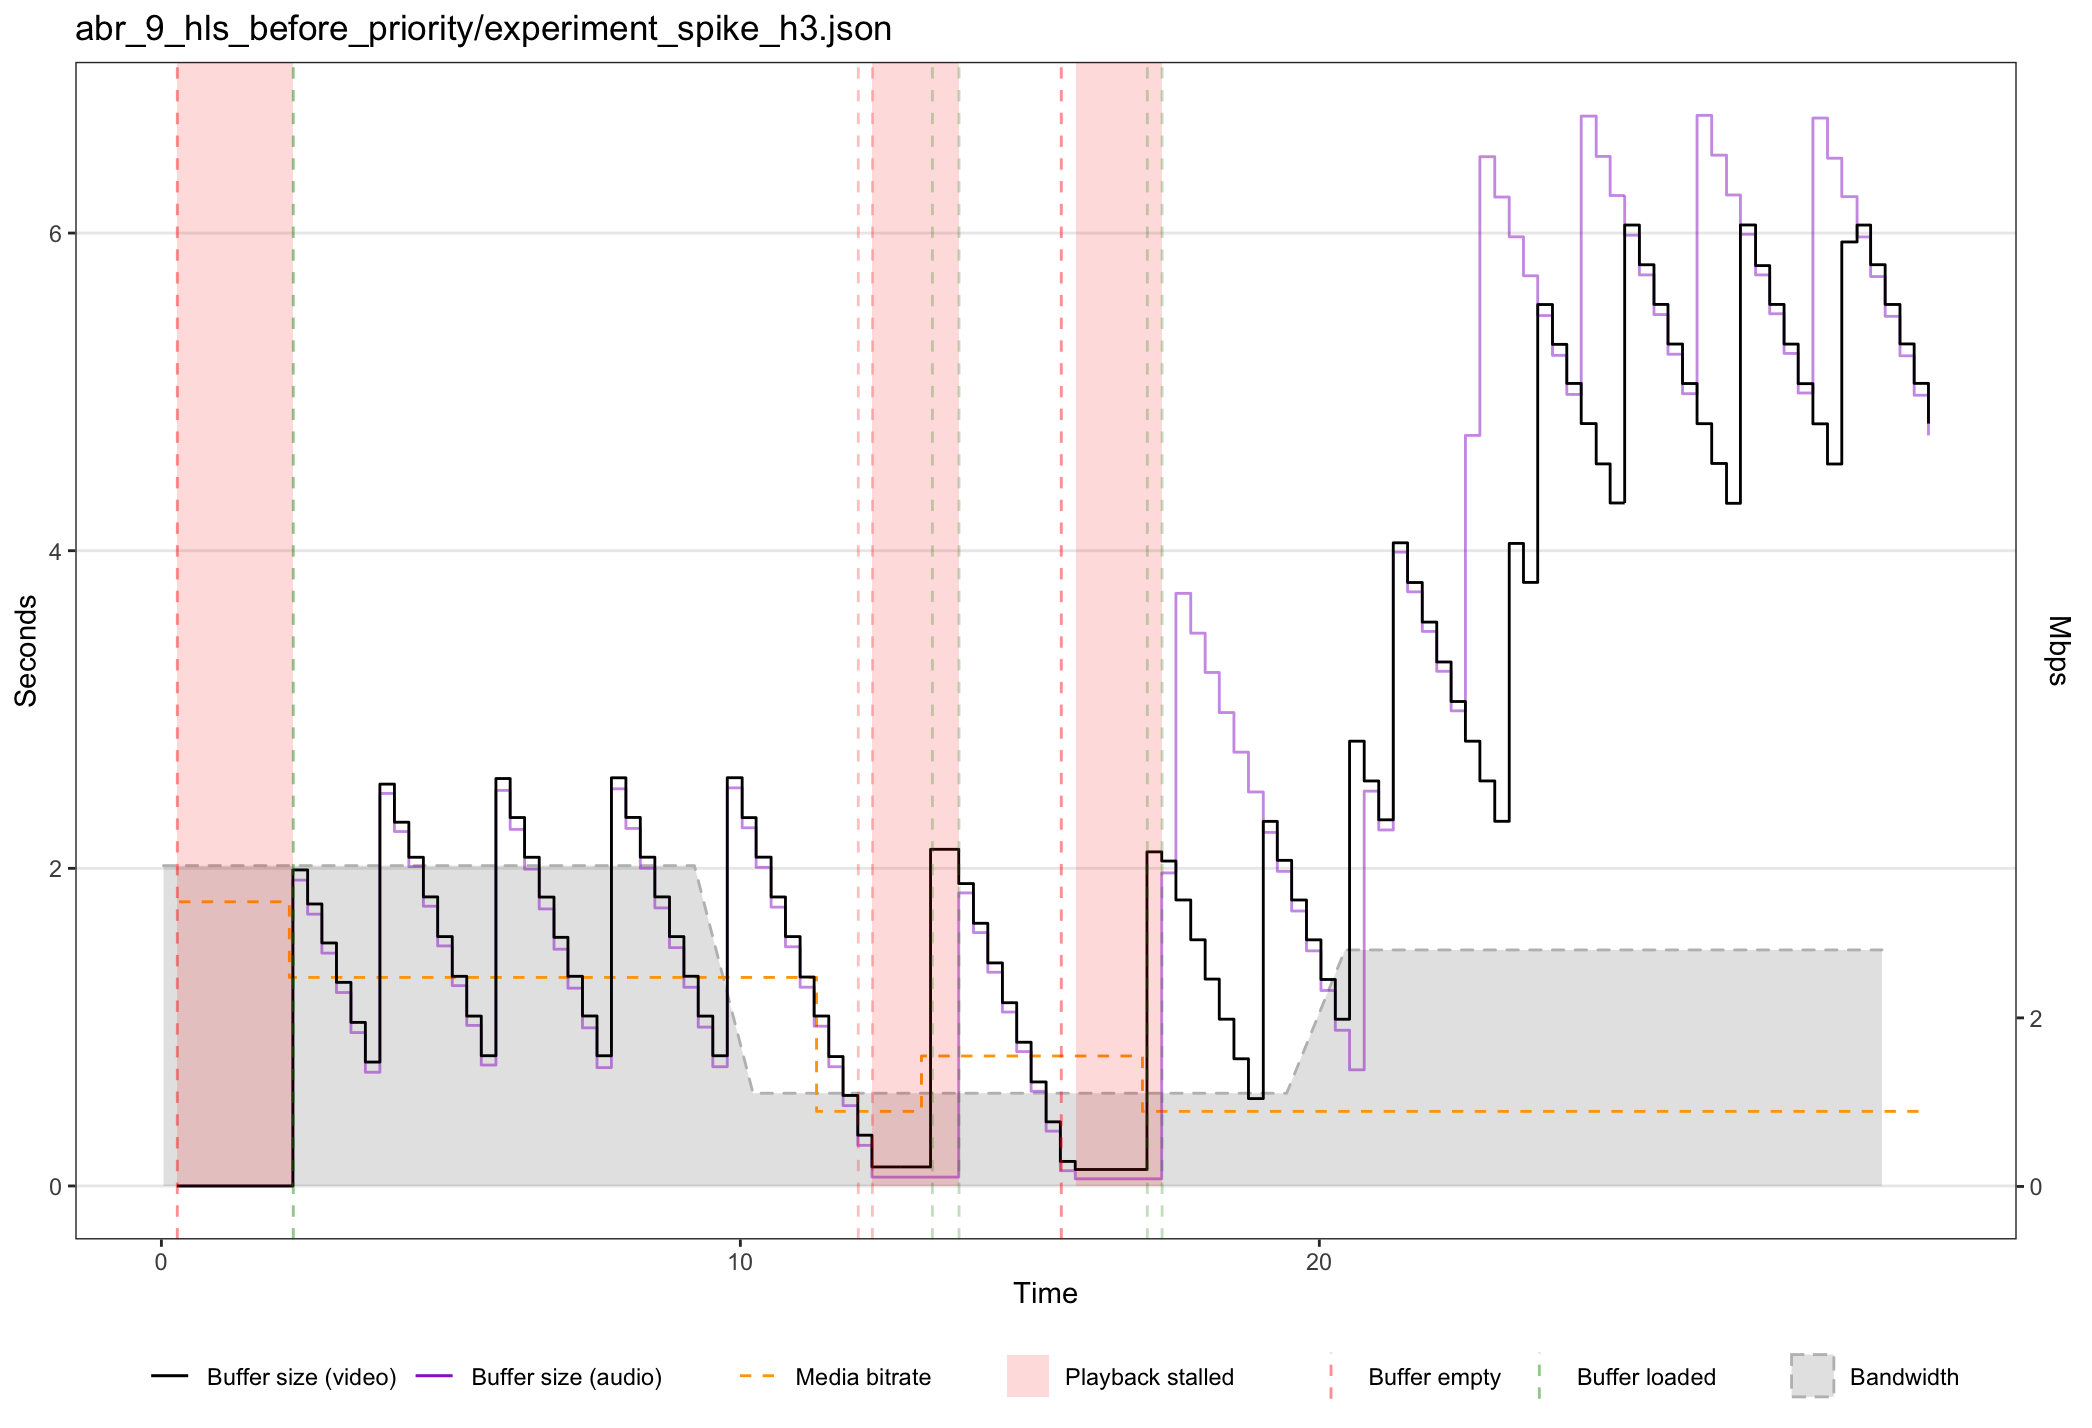
\includegraphics[width=0.9\textwidth]{res/eval_abr_spike_hls.png}
    \caption{HLS experiment over HTTP/3 with the \texttt{spike} network pattern.}
    \label{fig:eval_abr_hls}
\end{figure}

Finally, we also tested the behavior of the system when the \textbf{live catchup} feature is enabled. The live catchup feature increases the playback rate when the measured live latency is greater than the target one, up to a specified limit. In our tests, we used a maximum speed up of 1.5x. The results (not shown here) show that the live catchup indeed reduces the average latency, however seemingly causing additional playback stalls. The other obvious disadvantage is that for many types of video content having an increased playback rate is not an ideal experience.


